\chapter{基于纠删码对象存储的分布式文件存储}
\section{引言}
对于基于纠删码编码的分布式对象存储系统来说,由于纠删码编码和解码的计算开销很大,现有的分布式文件系统在对象存储上直接进行对象的修改操作,不仅会增加系统设计的复杂性,降低系统的通用性,而且由于在对象修改时需进行解码和编码,会导致系统的效率低下。因此,基于纠删码实现的对象存储一般假设对象是只读的,故并不能将存储系统中的对象直接封装为文件供分布式文件系统使用。

我们设计的基于纠删码的分布式文件系统以只读的对象存储系统为基础,将对文件的修改操作映射为对原始对象的修改事件,并将修改操作同样作为对象新增存储于对象存储引擎中,从而在逻辑上对原始对象进行了修改,简化了对象存储的设计,并减少了文件修改时的纠删码解码和重新编码的开销。此修改算法实现了文件的修改和附加等常见操作,从而可以基于此动态纠删码对象存储系统上实现典型的块存储、文件存储和数据库存储系统,以满足不同场景下的高性能高可用的分布式存储需求。
\section{基于纠删码的分布式存储系统}
\subsection{基于纠删码编码的对象存储}
在基于纠删码的分布式存储系统中,为了减少由于纠删码的编码和解码带来的计算开销,可以基于只读的分布式对象存储对数据进行存储。

对于待存储的对象,我们先使用 On-demand ARECS 算法选取校验码块数 $m$ 满足下式的纠删码编码方案 $(n+m,n)$:
$$
m(n)=\left\lceil\operatorname*{argmin}_{m}f(n,m)\right\rceil,\ \operatorname*{where}\ f(n,m) \geq 0
$$
再选取其中总读写时间 $t_{f}(n+m)$ 取最小值时的磁盘组:
$$
S_{d}'(n+m)=\operatorname*{argmin}_{S_{d}'(n+m)}\left(t_{calc}+\max_{d_{i}{\in}S_{d}'(n+m)}t_{d_i}+(r-1)\left(\max\left(t_{calc},\max_{d_{i}{\in}S_{d}'(n+m)}t_{d_i}\right)\right)\right)
$$

我们将待存储的数据对象分为 $n$ 份原始数据块,并使用里德-所罗门码纠删码编码生成 $m$ 份冗余备份块。对于这 $n+m$ 块数据,我们将其分别存放于选取的磁盘组 $S_{d}'(n+m)$ 中的 $n+m$ 块磁盘中。这样,我们便可以实现基于纠删码的快速的对象存储。

在数据的存储过程中,由于存储的数据块是只读的,因此每块数据块的长度是固定不变的。根据上一章中的研究,由于较大的对象在纠删码编码时存在由于编码矩阵过大,导致计算效率低下的问题,故在大对象存储时一般将其切分为较小的大小确定且均等的数据块。因此,我们在存储数据块时,可以不通过本地文件系统,直接将存储设备的线性地址空间分为若干个大小确定且均等的数据簇,每个数据簇存储一个数据块。这样,一个数据块就可以直接使用存储设备编号和数据簇编号来进行索引,避免了本地文件系统带来的性能损失,从而提高系统的并行性。
\subsection{基于对象存储的分布式文件系统中间件}
由于目前的分布式数据库以及云计算多需要一个支持修改操作的存储后端,上述只读的分布式对象存储不能满足这些存储领域的需求。因此,为了分布式存储系统的通用性,我们在基于纠删码实现的对象存储的基础上,设计了一个支持文件修改(Modify)和附加(Append)操作的存储引擎,来满足目前大型数据中心中多样化的存储需求。为了实现方便,此文件系统基于 Linux 的虚拟文件系统(Virtual File System,即 VFS)进行设计和实现。

VFS 子系统是 Linux 内核提供的一个灵活的文件系统框架\cite{wetzel2017virtual}。在 Linux 操作系统上,所有和文件系统相关的系统调用,均被提交至 VFS 子系统,由 VFS 子系统转发相应的内核模块。实际的文件系统模块可以是 ext4 或 XFS 等基于磁盘存储的文件系统,也可以是 proc 或 sysfs 等提供系统服务的虚拟的文件系统。我们通过实现一个新的虚拟文件系统模块作为中间件,截获 Linux 操作系统中应用程序的文件系统调用,再把其转换为基于纠删码的分布式对象存储系统的读写请求,使得各种 Linux 应用程序可以和使用原生文件系统一样,不做修改地支持分布式文件存储系统。

\begin{figure}[!htb]
\centering
\resizebox{.8\textwidth}{!}{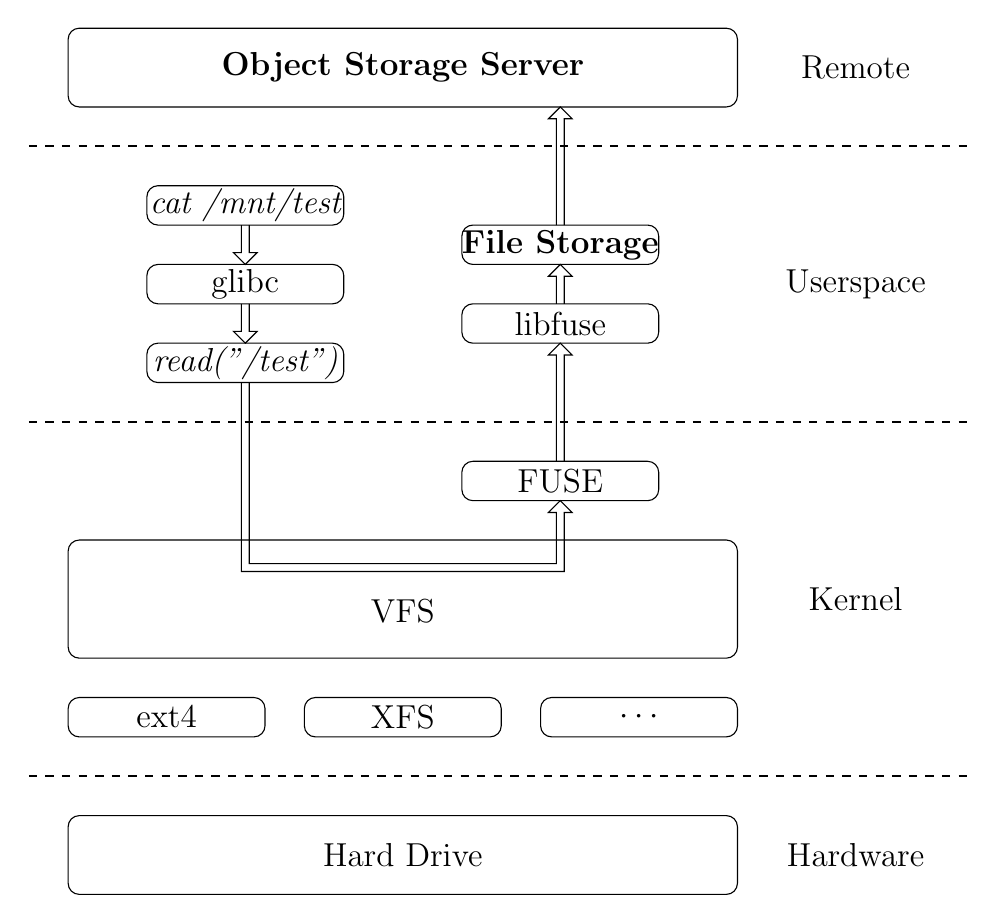
\begin{tikzpicture}
\fill [color=white,opacity=0] (0, 0) rectangle (12, 11);

\draw [rounded corners] (.5, 0) rectangle (9, 1);
\draw [dashed,thick] (0, 1.5) -- (12, 1.5);
\draw [rounded corners] (.5, 2) rectangle (3, 2.5);
\draw [rounded corners] (3.5, 2) rectangle (6, 2.5);
\draw [rounded corners] (6.5, 2) rectangle (9, 2.5);
\draw [rounded corners] (.5, 3) rectangle (9, 4.5);
\draw [rounded corners] (5.5, 5) rectangle (8, 5.5);
\draw [dashed,thick] (0, 6) -- (12, 6);
\draw [rounded corners] (1.5, 6.5) rectangle (4, 7);
\draw [rounded corners] (5.5, 7) rectangle (8, 7.5);
\draw [rounded corners] (1.5, 7.5) rectangle (4, 8);
\draw [rounded corners] (5.5, 8) rectangle (8, 8.5);
\draw [rounded corners] (1.5, 8.5) rectangle (4, 9);
\draw [dashed,thick] (0, 9.5) -- (12, 9.5);
\draw [rounded corners] (.5, 10) rectangle (9, 11);

\node at (10.5, .5) [font=\fontsize{12pt}{20pt}\selectfont] {Hardware};
\node at (10.5, 3.75) [font=\fontsize{12pt}{20pt}\selectfont] {Kernel};
\node at (10.5, 7.75) [font=\fontsize{12pt}{20pt}\selectfont] {Userspace};
\node at (10.5, 10.5) [font=\fontsize{12pt}{20pt}\selectfont] {Remote};

\node at (4.75, .5) [font=\fontsize{12pt}{20pt}\selectfont] {Hard Drive};
\node at (1.75, 2.25) [font=\fontsize{12pt}{20pt}\selectfont] {ext4};
\node at (4.75, 2.25) [font=\fontsize{12pt}{20pt}\selectfont] {XFS};
\node at (7.75, 2.25) [font=\fontsize{12pt}{20pt}\selectfont] {$\cdots$};
\node at (4.75, 3.6) [font=\fontsize{12pt}{20pt}\selectfont] {VFS};
\node at (6.75, 5.25) [font=\fontsize{12pt}{20pt}\selectfont] {FUSE};
\node at (2.75, 6.75) [font=\itshape\fontsize{12pt}{20pt}\selectfont] {read("/test")};
\node at (2.75, 7.75) [font=\fontsize{12pt}{20pt}\selectfont] {glibc};
\node at (2.75, 8.75) [font=\itshape\fontsize{12pt}{20pt}\selectfont] {cat /mnt/test};
\node at (6.75, 7.25) [font=\fontsize{12pt}{20pt}\selectfont] {libfuse};
\node at (6.75, 8.25) [font=\bfseries\fontsize{12pt}{20pt}\selectfont] {File Storage};
\node at (4.75, 10.5) [font=\bfseries\fontsize{12pt}{20pt}\selectfont] {Object Storage Server};

\draw (2.7, 8.5) -- (2.7, 8.15) -- (2.6, 8.15) -- (2.75, 8) -- (2.9, 8.15) -- (2.8, 8.15) -- (2.8, 8.5);
\draw (2.7, 7.5) -- (2.7, 7.15) -- (2.6, 7.15) -- (2.75, 7) -- (2.9, 7.15) -- (2.8, 7.15) -- (2.8, 7.5);
\draw (2.7, 6.5) -- (2.7, 4.1) -- (6.8, 4.1) -- (6.8, 4.85) -- (6.9, 4.85) -- (6.75, 5) -- (6.6, 4.85) -- (6.7, 4.85) -- (6.7, 4.2) -- (2.8, 4.2) -- (2.8, 6.5);
\draw (6.7, 5.5) -- (6.7, 6.85) -- (6.6, 6.85) -- (6.75, 7) -- (6.9, 6.85) -- (6.8, 6.85) -- (6.8, 5.5);
\draw (6.7, 7.5) -- (6.7, 7.85) -- (6.6, 7.85) -- (6.75, 8) -- (6.9, 7.85) -- (6.8, 7.85) -- (6.8, 7.5);
\draw (6.7, 8.5) -- (6.7, 9.85) -- (6.6, 9.85) -- (6.75, 10) -- (6.9, 9.85) -- (6.8, 9.85) -- (6.8, 8.5);
\end{tikzpicture}
}
\caption{基于 FUSE 框架实现的文件系统架构图}
\label{p3}
\end{figure}

在基于 Linux 虚拟文件系统的分布式文件系统接口实现中,我们采用了用户空间文件系统(Filesystem in Userspace,即 FUSE)框架,如图 \ref{p3} 所示。我们通过 FUSE 在用户态创建了一个分布式文件系统的服务进程,实现文件系统的标准 POSIX 接口,并将其转换为基于纠删码的分布式对象存储系统的读写请求调用。此文件系统主要分为两大部分,文件系统的元数据和文件内容数据。类似于分布式文件系统 Ceph 的方案,我们将元数据存储和文件内容数据存储分离,元数据采取单独的存储池和数据结构进行存储,文件内容数据作为对象存储于分布式对象存储系统中。

在分布式文件系统的元数据存储部分,我们存储的分布式文件系统元数据包含文件的修改时间和权限等属性信息,以及文件在分布式对象存储中的对象索引列表。由于分布式文件系统的元数据在文件的 I/O 操作中需要频繁读写,因此在分布式文件系统进行挂载时,服务进程通过对文件系统的元数据进行本地缓存,从而优化文件的读写速度,保障文件系统元数据的快速读写。

在分布式文件系统的文件内容数据存储部分,我们使用修改事件存储文件的内容数据。在文件每次进行创建和修改时,将其新增或修改的内容均单独作为一个对象,给予编号存储于分布式对象存储中。在文件进行读取时,通过寻找读取位置最近的修改记录,确定待读取数据所位于的对象。通过这种方式,我们避免了在文件每次进行修改的重新编码和解码操作,从而提高系统效率。
\section{基于修改事件的分布式文件修改算法}
\subsection{基于修改事件的文件数据存储结构}
对于基于修改事件的分布式文件系统,在文件创建、修改或附加等事件发生时,我们将每个修改事件均描述为一个修改事件。下面我们详细介绍修改事件的存储方式。
\subsubsection{随机对象唯一编号的生成方案}
首先,我们需要为每个修改事件均分配一个随机的对象唯一编号,在此记为 UUID。由于在文件读取时需要获知文件修改的先后顺序,从而确定最近的修改记录,因此 UUID 需要包含修改事件的高精度时间。为了保证系统的通用性,我们不妨使用根据 RFC 4122 标准生成的 UUID,其结构如图 \ref{p16} 所示。在 UUID 的生成中,我们采用的版本号为 1,变体号为 1,时间戳是一个 60 比特的数据,记录从协调世界时(Coordinated Universal Time,即 UTC)1582 年 10 月 15 日 00 时 00 分 00 秒(即首次采用格里高利历的日期)至今所经过的 100 纳秒数,时钟序列是一个 14 比特的数据,在系统时间戳倒退时进行相应的增加,节点则是一个 48 比特的数据,存储当前节点编号,通常使用网卡的物理地址(Media Access Control Address,即 MAC 地址)。

\begin{figure}[!htb]
\centering
\resizebox{.8\textwidth}{!}{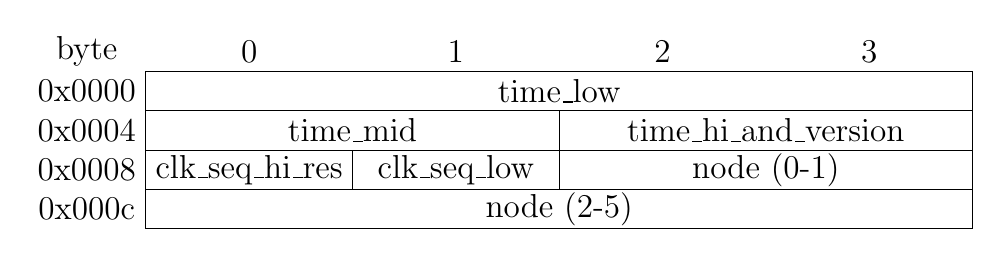
\begin{tikzpicture}
\newcommand\tablewidth{10.5}
\newcommand\tablex{1.5}
\fill [color=white,opacity=0] (0, 0) rectangle (12, -2.5);

\draw (\tablex, -.5) -- (12, -.5) -- (12, -2.5) -- (\tablex, -2.5) -- cycle;

\node at (\tablex/2, -.25) [font=\fontsize{12pt}{20pt}\selectfont] {byte};
\foreach \x in {0,...,3} {
    \node at (\x/4*\tablewidth+\tablewidth/8+\tablex, -.25) [font=\fontsize{12pt}{20pt}\selectfont] {\x};
}
\node at (\tablex/2, -.75) [font=\fontsize{12pt}{20pt}\selectfont] {0x0000};
\node at (6+\tablex/2, -.75) [font=\fontsize{12pt}{20pt}\selectfont] {time\_low};
\draw (\tablex, -1) -- (12, -1);
\node at (\tablex/2, -1.25) [font=\fontsize{12pt}{20pt}\selectfont] {0x0004};
\draw (6+\tablex/2, -1) -- (6+\tablex/2, -2);
\node at (3+\tablex*3/4, -1.25) [font=\fontsize{12pt}{20pt}\selectfont] {time\_mid};
\node at (9+\tablex/4, -1.25) [font=\fontsize{12pt}{20pt}\selectfont] {time\_hi\_and\_version};
\draw (\tablex, -1.5) -- (12, -1.5);
\node at (\tablex/2, -1.75) [font=\fontsize{12pt}{20pt}\selectfont] {0x0008};
\draw (3+\tablex*3/4, -1.5) -- (3+\tablex*3/4, -2);
\node at (1.5+\tablex*7/8, -1.75) [font=\fontsize{12pt}{20pt}\selectfont] {clk\_seq\_hi\_res};
\node at (4.5+\tablex*5/8, -1.75) [font=\fontsize{12pt}{20pt}\selectfont] {clk\_seq\_low};
\node at (9+\tablex/4, -1.75) [font=\fontsize{12pt}{20pt}\selectfont] {node (0-1)};
\draw (\tablex, -2) -- (12, -2);
\node at (\tablex/2, -2.25) [font=\fontsize{12pt}{20pt}\selectfont] {0x000c};
\node at (6+\tablex/2, -2.25) [font=\fontsize{12pt}{20pt}\selectfont] {node (2-5)};
\end{tikzpicture}
}
\caption{对象唯一编号结构示意图}
\label{p16}
\end{figure}
\subsubsection{文件修改对象示意}
在按照 RFC 4122 标准生成 UUID 作为对象的唯一编号之后,我们将修改的后的文件内容作为单独的对象,以生成的唯一编号 UUID 作为索引,存储于基于纠删码的对象存储系统中。对于文件修改和文件附加操作,存储的对象相对于原始文件示意如图 \ref{p4} 所示。

\begin{figure}[!htb]
\centering
\resizebox{.8\textwidth}{!}{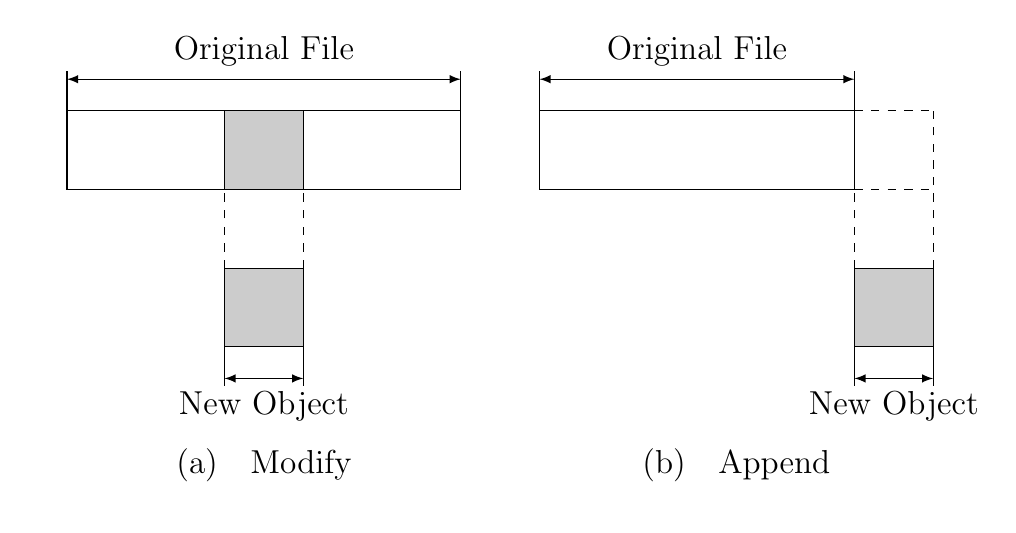
\begin{tikzpicture}
\fill [color=white,opacity=0] (0, 0) rectangle (12, 6);

\node at (3, 0.5) [font=\fontsize{12pt}{20pt}\selectfont] {(a){\quad}Modify};
\node at (3, 1.25) [font=\fontsize{12pt}{20pt}\selectfont] {New Object};
\draw (2.5, 2) -- (2.5, 1.5);
\draw (3.5, 2) -- (3.5, 1.5);
\draw [latex-latex] (2.5, 1.6) -- (3.5, 1.6);
\filldraw [fill=black!20!white] (2.5, 2) rectangle (3.5, 3);
\draw [dashed] (2.5, 3) -- (2.5, 4);
\draw [dashed] (3.5, 3) -- (3.5, 4);
\fill [color=black!20!white] (2.5, 4) rectangle (3.5, 5);
\draw (0.5, 4) rectangle (5.5, 5);
\draw (2.5, 4) -- (2.5, 5);
\draw (3.5, 4) -- (3.5, 5);
\draw (0.5, 5) -- (0.5, 5.5);
\draw (5.5, 5) -- (5.5, 5.5);
\draw [latex-latex] (0.5, 5.4) -- (5.5, 5.4);
\node at (3, 5.75) [font=\fontsize{12pt}{20pt}\selectfont] {Original File};

\node at (9, 0.5) [font=\fontsize{12pt}{20pt}\selectfont] {(b){\quad}Append};
\node at (11, 1.25) [font=\fontsize{12pt}{20pt}\selectfont] {New Object};
\draw (10.5, 2) -- (10.5, 1.5);
\draw (11.5, 2) -- (11.5, 1.5);
\draw [latex-latex] (10.5, 1.6) -- (11.5, 1.6);
\filldraw [fill=black!20!white] (10.5, 2) rectangle (11.5, 3);
\draw [dashed] (10.5, 3) -- (10.5, 4);
\draw [dashed] (11.5, 3) -- (11.5, 5);
\draw (6.5, 4) rectangle (10.5, 5);
\draw [dashed] (10.5, 4) -- (11.5, 4);
\draw [dashed] (10.5, 5) -- (11.5, 5);
\draw (6.5, 5) -- (6.5, 5.5);
\draw (10.5, 5) -- (10.5, 5.5);
\draw [latex-latex] (6.5, 5.4) -- (10.5, 5.4);
\node at (8.5, 5.75) [font=\fontsize{12pt}{20pt}\selectfont] {Original File};
\end{tikzpicture}
}
\caption{修改事件对象示意}
\label{p4}
\end{figure}
\subsubsection{文件元数据的存储结构}
对于存储的文件修改对象,我们需要在分布式文件系统的元数据中对其进行索引。我们首先需要在元数据中存储此次修改事件内容的编号 UUID,从而记录文件变更后的内容。此外,我们还需要存储此变更所参照的原始文件,即编号 UUID$_{prev}$,从而确定文件修改的参照点。我们还需要记录此修改或者附加的起始位置 start $=$ offset 和终止位置 end $=$ offset $+$ length,其中 length 为编号 UUID 所对应的对象大小。我们采用如图 \ref{p15} 的结构存储这些数据,从而得到一个完整的文件修改记录,并计算文件的最新内容。

\begin{figure}[!htb]
\centering
\resizebox{.8\textwidth}{!}{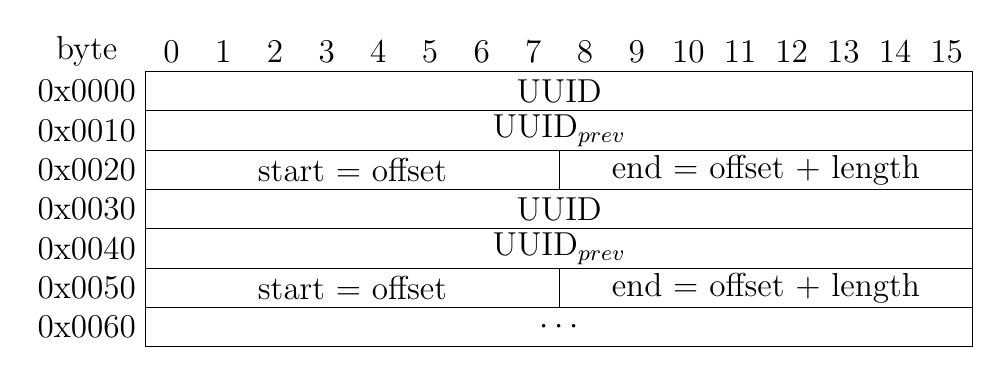
\begin{tikzpicture}
\newcommand\tablewidth{10.5}
\newcommand\tablex{1.5}
\fill [color=white,opacity=0] (0, 0) rectangle (12, -4);

\draw (\tablex, -.5) -- (12, -.5) -- (12, -4) -- (\tablex, -4) -- cycle;

\node at (\tablex/2, -.25) [font=\fontsize{12pt}{20pt}\selectfont] {byte};
\foreach \x in {0,...,15} {
    \node at (\x/16*\tablewidth+\tablewidth/32+\tablex, -.25) [font=\fontsize{12pt}{20pt}\selectfont] {\x};
}
\draw (\tablex, -1) -- (12, -1);
\node at (\tablex/2, -.75) [font=\fontsize{12pt}{20pt}\selectfont] {0x0000};
\node at (6+\tablex/2, -.75) [font=\fontsize{12pt}{20pt}\selectfont] {UUID};
\draw (\tablex, -1.5) -- (12, -1.5);
\node at (\tablex/2, -1.25) [font=\fontsize{12pt}{20pt}\selectfont] {0x0010};
\node at (6+\tablex/2, -1.25) [font=\fontsize{12pt}{20pt}\selectfont] {UUID$_{prev}$};
\draw (\tablex, -2) -- (12, -2);
\draw (6+\tablex/2, -1.5) -- (6+\tablex/2, -2);
\node at (\tablex/2, -1.75) [font=\fontsize{12pt}{20pt}\selectfont] {0x0020};
\node at (3+\tablex*3/4, -1.75) [font=\fontsize{12pt}{20pt}\selectfont] {start $=$ offset};
\node at (9+\tablex/4, -1.75) [font=\fontsize{12pt}{20pt}\selectfont] {end $=$ offset $+$ length};

\draw (\tablex, -2.5) -- (12, -2.5);
\node at (\tablex/2, -2.25) [font=\fontsize{12pt}{20pt}\selectfont] {0x0030};
\node at (6+\tablex/2, -2.25) [font=\fontsize{12pt}{20pt}\selectfont] {UUID};
\draw (\tablex, -3) -- (12, -3);
\node at (\tablex/2, -2.75) [font=\fontsize{12pt}{20pt}\selectfont] {0x0040};
\node at (6+\tablex/2, -2.75) [font=\fontsize{12pt}{20pt}\selectfont] {UUID$_{prev}$};
\draw (\tablex, -3.5) -- (12, -3.5);
\draw (6+\tablex/2, -3) -- (6+\tablex/2, -3.5);
\node at (\tablex/2, -3.25) [font=\fontsize{12pt}{20pt}\selectfont] {0x0050};
\node at (3+\tablex*3/4, -3.25) [font=\fontsize{12pt}{20pt}\selectfont] {start $=$ offset};
\node at (9+\tablex/4, -3.25) [font=\fontsize{12pt}{20pt}\selectfont] {end $=$ offset $+$ length};

\node at (\tablex/2, -3.75) [font=\fontsize{12pt}{20pt}\selectfont] {0x0060};
\node at (6+\tablex/2, -3.75) [font=\fontsize{12pt}{20pt}\selectfont] {$\cdots$};

\end{tikzpicture}
}
\caption{分布式文件系统的元数据结构}
\label{p15}
\end{figure}

在读取文件时,我们可以遍历这个元数据结构,选择所有 UUID 编号中时间戳和时钟序列最新的对象,来确定当前最新版本的文件。若文件待读取的位置不在上述 UUID 对应记录的 start 和 end 之间,则递归地按上述步骤读取 UUID$_{prev}$ 对应的记录,直至找到符合条件的记录,并返回符合条件的记录的 UUID 对应的对象中的相应位置。此算法流程图如 \ref{p21} 所示。

\begin{figure}[!htb]
\centering
\resizebox{.8\textwidth}{!}{\begin{tikzpicture}
\fill [color=white,opacity=0] (0, 0) rectangle (12, -15);

\node at (6, -0.5) [font=\fontsize{12pt}{20pt}\selectfont] {读取文件 pos 位置内容};
\draw (9, 0) arc (90:-90:0.5) -- (3, -1) arc (270:90:0.5) -- cycle;
\node at (6, -3) [align=center,font=\fontsize{12pt}{20pt}\selectfont] {令变量 UUID、prev、start、end 为待读取文\\件元数据中 UUID 时间戳最近的记录的对应值};
\draw (1, -2) rectangle (11, -4);
\node at (6, -6) [font=\fontsize{12pt}{20pt}\selectfont] {start $\leq$ pos $<$ end $?$};
\draw (6, -5) -- (9, -6) -- (6, -7) -- (3, -6) -- cycle;
\node at (6, -8) [font=\fontsize{12pt}{20pt}\selectfont] {否};
\node at (11.75, -8) [font=\fontsize{12pt}{20pt}\selectfont] {是};
\node at (6, -10) [align=center,font=\fontsize{12pt}{20pt}\selectfont] {令变量 UUID、prev、start、end 为待读取\\文件元数据中 UUID 为 prev 的记录的对应值};
\draw (1, -9) rectangle (11, -11);
\node at (6, -14) [align=center,font=\fontsize{12pt}{20pt}\selectfont] {返回对象存储中 UUID 对应对\\象的 $($pos $-$ start$)$ 位置的数据};
\draw (9, -13) arc (90:-90:1) -- (3, -15) arc (270:90:1) -- cycle;

\newcommand\arrowhead{0.15}
\draw (6, -1) -- (6, -2+\arrowhead);
\fill [color=black] (6-\arrowhead, -2+\arrowhead) -- (6, -2) -- (6+\arrowhead, -2+\arrowhead);
\draw (6, -4) -- (6, -5+\arrowhead);
\fill [color=black] (6-\arrowhead, -5+\arrowhead) -- (6, -5) -- (6+\arrowhead, -5+\arrowhead);
\draw (6, -7) -- (6, -7.75);
\draw (6, -8.25) -- (6, -9+\arrowhead);
\fill [color=black] (6-\arrowhead, -9+\arrowhead) -- (6, -9) -- (6+\arrowhead, -9+\arrowhead);
\draw (9, -6) -- (11.75, -6) -- (11.75, -7.75);
\draw (11.75, -8.25) -- (11.75, -12) -- (6, -12) -- (6, -13+\arrowhead);
\fill [color=black] (6-\arrowhead, -13+\arrowhead) -- (6, -13) -- (6+\arrowhead, -13+\arrowhead);
\draw (1, -10) -- (0.25, -10) -- (0.25, -6) -- (3-\arrowhead, -6);
\fill [color=black] (3-\arrowhead, -6-\arrowhead) -- (3, -6) -- (3-\arrowhead, -6+\arrowhead);
\end{tikzpicture}
}
\caption{文件读取流程图}
\label{p21}
\end{figure}
\subsubsection{文件的版本历史和并发写入}
通过上述文件修改事件结构,我们可以维护一个文件的历史版本记录,在文件打开操作时,我们确定一个最新的文件版本,在此后对该文件的操作中,均针对此版本的文件进行修改,因此可以保证并发的写入请求不发生冲突。如果存在多个进程同时操作同一个文件,便会在文件系统中同时存储该文件的多个版本,文件系统将选择最新修改的文件版本。
\subsection{文件修改事件元数据的无锁更新算法}
在元数据的修改过程中,为了保证数组的一致性,若有多个线程同时对数组进行更新,则可能导致数据的不一致。为了防止对共享数据的非法访问,一般可以采用自旋锁等结构对并发访问进行限制。但采用锁机制会产生额外的性能开销。由于我们的数据结构和访问模式较为固定,在此处我们采用基于数组的无锁队列进行元数据的更新。
\subsubsection{无锁队列的结构}
在基于数组的无锁队列中,我们采用数组下标 $read\_index$ 和 $write\_index$ 来分别表示当前数组的读下标和写下标。在数据初始化时,这两个下标均初始化为 0,即数据的第一个元素位置。在数据插入时,我们使用原子操作,将 $write\_index$ 加 1,并返回原来的 $write\_index$ 值作为写入位置 $write\_current$。之后我们便可以向数组的 $write\_current$ 位置写入数据。在数据写入完成后,我们使用原子操作,比较若 $read\_index$ 与 $write\_current$ 相同,则将 $read\_index$ 改为 $write\_current+1$,否则不进行任何操作。若执行此步骤后 $read\_index \leq write\_current$,则重新执行上面一步,直至 $read\_index>write\_current$。整个数据插入过程如图 \ref{p19} 所示。

\begin{figure}[!htb]
\centering
\resizebox{.8\textwidth}{!}{\begin{tikzpicture}
\fill [color=white,opacity=0] (0, 0) rectangle (12, -10);

\node at (0.4, -1.25) [font=\fontsize{12pt}{20pt}\selectfont] {(1)};
\node at (9.6, -1.25) [font=\fontsize{12pt}{20pt}\selectfont] {初始状态};
\draw (1.2, -0.9) rectangle (6.8, -1.6);
\draw (2, -0.9) -- (2, -1.6);
\draw (2.8, -0.9) -- (2.8, -1.6);
\draw (3.6, -0.9) -- (3.6, -1.6);
\draw (4.4, -0.9) -- (4.4, -1.6);
\draw (5.2, -0.9) -- (5.2, -1.6);
\draw (6, -0.9) -- (6, -1.6);
\draw (1.2, -0.9) -- (2, -1.6);
\draw (1.2, -1.6) -- (2, -0.9);
\draw (2, -0.9) -- (2.8, -1.6);
\draw (2, -1.6) -- (2.8, -0.9);
\node at (3.2, -0.25) [font=\fontsize{12pt}{20pt}\selectfont] {$read\_index$};
\node at (3.2, -2.25) [font=\fontsize{12pt}{20pt}\selectfont] {$write\_index$};
\draw [-latex] (3.2, -0.5) -- (3.2, -0.9);
\draw [-latex] (3.2, -2) -- (3.2, -1.6);
\node at (0.4, -3.75) [font=\fontsize{12pt}{20pt}\selectfont] {(2)};
\node at (9.6, -3.75) [font=\fontsize{12pt}{20pt}\selectfont] {申请空间(原子操作)};
\draw (1.2, -3.4) rectangle (6.8, -4.1);
\draw (2, -3.4) -- (2, -4.1);
\draw (2.8, -3.4) -- (2.8, -4.1);
\draw (3.6, -3.4) -- (3.6, -4.1);
\draw (4.4, -3.4) -- (4.4, -4.1);
\draw (5.2, -3.4) -- (5.2, -4.1);
\draw (6, -3.4) -- (6, -4.1);
\draw (1.2, -3.4) -- (2, -4.1);
\draw (1.2, -4.1) -- (2, -3.4);
\draw (2, -3.4) -- (2.8, -4.1);
\draw (2, -4.1) -- (2.8, -3.4);
\node at (3.2, -2.75) [font=\fontsize{12pt}{20pt}\selectfont] {$read\_index$};
\node at (4, -4.75) [font=\fontsize{12pt}{20pt}\selectfont] {$write\_index$};
\draw [-latex] (3.2, -3) -- (3.2, -3.4);
\draw [-latex] (4, -4.5) -- (4, -4.1);
\node at (0.4, -6.25) [font=\fontsize{12pt}{20pt}\selectfont] {(3)};
\node at (9.6, -6.25) [font=\fontsize{12pt}{20pt}\selectfont] {写入数据};
\draw (1.2, -5.9) rectangle (6.8, -6.6);
\draw (2, -5.9) -- (2, -6.6);
\draw (2.8, -5.9) -- (2.8, -6.6);
\draw (3.6, -5.9) -- (3.6, -6.6);
\draw (4.4, -5.9) -- (4.4, -6.6);
\draw (5.2, -5.9) -- (5.2, -6.6);
\draw (6, -5.9) -- (6, -6.6);
\draw (1.2, -5.9) -- (2, -6.6);
\draw (1.2, -6.6) -- (2, -5.9);
\draw (2, -5.9) -- (2.8, -6.6);
\draw (2, -6.6) -- (2.8, -5.9);
\draw (2.8, -5.9) -- (3.6, -6.6);
\draw (2.8, -6.6) -- (3.6, -5.9);
\node at (3.2, -5.25) [font=\fontsize{12pt}{20pt}\selectfont] {$read\_index$};
\node at (4, -7.25) [font=\fontsize{12pt}{20pt}\selectfont] {$write\_index$};
\draw [-latex] (3.2, -5.5) -- (3.2, -5.9);
\draw [-latex] (4, -7) -- (4, -6.6);
\node at (0.4, -8.75) [font=\fontsize{12pt}{20pt}\selectfont] {(4)};
\node at (9.6, -8.75) [font=\fontsize{12pt}{20pt}\selectfont] {完成写入(原子操作)};
\draw (1.2, -8.4) rectangle (6.8, -9.1);
\draw (2, -8.4) -- (2, -9.1);
\draw (2.8, -8.4) -- (2.8, -9.1);
\draw (3.6, -8.4) -- (3.6, -9.1);
\draw (4.4, -8.4) -- (4.4, -9.1);
\draw (5.2, -8.4) -- (5.2, -9.1);
\draw (6, -8.4) -- (6, -9.1);
\draw (1.2, -8.4) -- (2, -9.1);
\draw (1.2, -9.1) -- (2, -8.4);
\draw (2, -8.4) -- (2.8, -9.1);
\draw (2, -9.1) -- (2.8, -8.4);
\draw (2.8, -8.4) -- (3.6, -9.1);
\draw (2.8, -9.1) -- (3.6, -8.4);
\node at (4, -7.75) [font=\fontsize{12pt}{20pt}\selectfont] {$read\_index$};
\node at (4, -9.75) [font=\fontsize{12pt}{20pt}\selectfont] {$write\_index$};
\draw [-latex] (4, -8) -- (4, -8.4);
\draw [-latex] (4, -9.5) -- (4, -9.1);
\end{tikzpicture}
}
\caption{无锁队列的数据插入示意}
\label{p19}
\end{figure}
\subsubsection{无锁队列的并发插入}
通过采用此无锁队列,我们在更新对象元数据时,可以直接将修改对象的编号等信息插入到元数据末端。在多个进程进行并发写入时,此队列可以做到无锁的并发写入,如图 \ref{p20} 所示,在一个进程完成数据写入之前,又有另一个进程申请写入数据。对于这种情况,基于数组的无锁队列中的 $write\_current$ 向前继续移动一个元素,然后两个进程可以分别在对应位置写入,不会造成冲突。在数据写入完成之后,在对 $read\_index$ 递增时,第二个写入进程必须等待第一个写入进程完成之后才能进行递增,因为我们必须保证数据完全被写入后才能被读取。基于此无锁队列的元数据存储在读取文件时,即进行元数据遍历等读取操作时,可以读取的数据便是无锁队列中已经完成写入的数据,也就是从上述队列头部开始,到 $read\_index$ 前的位置为止之间的数据。

\begin{figure}[!htb]
\centering
\resizebox{.8\textwidth}{!}{\begin{tikzpicture}
\fill [color=white,opacity=0] (0, 0) rectangle (12, -15);

\node at (0.4, -1.25) [font=\fontsize{12pt}{20pt}\selectfont] {(1)};
\node at (9.6, -1.25) [font=\fontsize{12pt}{20pt}\selectfont] {初始状态};
\draw (1.2, -0.9) rectangle (6.8, -1.6);
\draw (2, -0.9) -- (2, -1.6);
\draw (2.8, -0.9) -- (2.8, -1.6);
\draw (3.6, -0.9) -- (3.6, -1.6);
\draw (4.4, -0.9) -- (4.4, -1.6);
\draw (5.2, -0.9) -- (5.2, -1.6);
\draw (6, -0.9) -- (6, -1.6);
\draw (1.2, -0.9) -- (2, -1.6);
\draw (1.2, -1.6) -- (2, -0.9);
\draw (2, -0.9) -- (2.8, -1.6);
\draw (2, -1.6) -- (2.8, -0.9);
\draw (2.8, -0.9) -- (3.6, -1.6);
\draw (2.8, -1.6) -- (3.6, -0.9);
\node at (4, -0.25) [font=\fontsize{12pt}{20pt}\selectfont] {$read\_index$};
\node at (4, -2.25) [font=\fontsize{12pt}{20pt}\selectfont] {$write\_index$};
\draw [-latex] (4, -0.5) -- (4, -0.9);
\draw [-latex] (4, -2) -- (4, -1.6);
\node at (0.4, -3.75) [font=\fontsize{12pt}{20pt}\selectfont] {(2)};
\node at (9.6, -3.75) [align=center,font=\fontsize{12pt}{20pt}\selectfont] {进程 A 申请空间\\(原子操作)};
\draw (1.2, -3.4) rectangle (6.8, -4.1);
\draw (2, -3.4) -- (2, -4.1);
\draw (2.8, -3.4) -- (2.8, -4.1);
\draw (3.6, -3.4) -- (3.6, -4.1);
\draw (4.4, -3.4) -- (4.4, -4.1);
\draw (5.2, -3.4) -- (5.2, -4.1);
\draw (6, -3.4) -- (6, -4.1);
\draw (1.2, -3.4) -- (2, -4.1);
\draw (1.2, -4.1) -- (2, -3.4);
\draw (2, -3.4) -- (2.8, -4.1);
\draw (2, -4.1) -- (2.8, -3.4);
\draw (2.8, -3.4) -- (3.6, -4.1);
\draw (2.8, -4.1) -- (3.6, -3.4);
\node at (4, -2.75) [font=\fontsize{12pt}{20pt}\selectfont] {$read\_index$};
\node at (4.8, -4.75) [font=\fontsize{12pt}{20pt}\selectfont] {$write\_index$};
\draw [-latex] (4, -3) -- (4, -3.4);
\draw [-latex] (4.8, -4.5) -- (4.8, -4.1);
\node at (0.4, -6.25) [font=\fontsize{12pt}{20pt}\selectfont] {(3)};
\node at (9.6, -6.25) [align=center,font=\fontsize{12pt}{20pt}\selectfont] {进程 B 申请空间\\(原子操作)};
\draw (1.2, -5.9) rectangle (6.8, -6.6);
\draw (2, -5.9) -- (2, -6.6);
\draw (2.8, -5.9) -- (2.8, -6.6);
\draw (3.6, -5.9) -- (3.6, -6.6);
\draw (4.4, -5.9) -- (4.4, -6.6);
\draw (5.2, -5.9) -- (5.2, -6.6);
\draw (6, -5.9) -- (6, -6.6);
\draw (1.2, -5.9) -- (2, -6.6);
\draw (1.2, -6.6) -- (2, -5.9);
\draw (2, -5.9) -- (2.8, -6.6);
\draw (2, -6.6) -- (2.8, -5.9);
\draw (2.8, -5.9) -- (3.6, -6.6);
\draw (2.8, -6.6) -- (3.6, -5.9);
\node at (4, -5.25) [font=\fontsize{12pt}{20pt}\selectfont] {$read\_index$};
\node at (5.6, -7.25) [font=\fontsize{12pt}{20pt}\selectfont] {$write\_index$};
\draw [-latex] (4, -5.5) -- (4, -5.9);
\draw [-latex] (5.6, -7) -- (5.6, -6.6);
\node at (0.4, -8.75) [font=\fontsize{12pt}{20pt}\selectfont] {(4)};
\node at (9.6, -8.75) [align=center,font=\fontsize{12pt}{20pt}\selectfont] {进程 A 写入数据;\\进程 B 写入数据};
\draw (1.2, -8.4) rectangle (6.8, -9.1);
\draw (2, -8.4) -- (2, -9.1);
\draw (2.8, -8.4) -- (2.8, -9.1);
\draw (3.6, -8.4) -- (3.6, -9.1);
\draw (4.4, -8.4) -- (4.4, -9.1);
\draw (5.2, -8.4) -- (5.2, -9.1);
\draw (6, -8.4) -- (6, -9.1);
\draw (1.2, -8.4) -- (2, -9.1);
\draw (1.2, -9.1) -- (2, -8.4);
\draw (2, -8.4) -- (2.8, -9.1);
\draw (2, -9.1) -- (2.8, -8.4);
\draw (2.8, -8.4) -- (3.6, -9.1);
\draw (2.8, -9.1) -- (3.6, -8.4);
\draw (3.6, -8.4) -- (4.4, -9.1);
\draw (3.6, -9.1) -- (4.4, -8.4);
\draw (4.4, -8.4) -- (5.2, -9.1);
\draw (4.4, -9.1) -- (5.2, -8.4);
\node at (4, -7.75) [font=\fontsize{12pt}{20pt}\selectfont] {$read\_index$};
\node at (5.6, -9.75) [font=\fontsize{12pt}{20pt}\selectfont] {$write\_index$};
\draw [-latex] (4, -8) -- (4, -8.4);
\draw [-latex] (5.6, -9.5) -- (5.6, -9.1);
\node at (0.4, -11.25) [font=\fontsize{12pt}{20pt}\selectfont] {(5)};
\node at (9.6, -11.25) [align=center,font=\fontsize{12pt}{20pt}\selectfont] {进程 B 等待;进程 A\\完成写入(原子操作)};
\draw (1.2, -10.9) rectangle (6.8, -11.6);
\draw (2, -10.9) -- (2, -11.6);
\draw (2.8, -10.9) -- (2.8, -11.6);
\draw (3.6, -10.9) -- (3.6, -11.6);
\draw (4.4, -10.9) -- (4.4, -11.6);
\draw (5.2, -10.9) -- (5.2, -11.6);
\draw (6, -10.9) -- (6, -11.6);
\draw (1.2, -10.9) -- (2, -11.6);
\draw (1.2, -11.6) -- (2, -10.9);
\draw (2, -10.9) -- (2.8, -11.6);
\draw (2, -11.6) -- (2.8, -10.9);
\draw (2.8, -10.9) -- (3.6, -11.6);
\draw (2.8, -11.6) -- (3.6, -10.9);
\draw (3.6, -10.9) -- (4.4, -11.6);
\draw (3.6, -11.6) -- (4.4, -10.9);
\draw (4.4, -10.9) -- (5.2, -11.6);
\draw (4.4, -11.6) -- (5.2, -10.9);
\node at (4.8, -10.25) [font=\fontsize{12pt}{20pt}\selectfont] {$read\_index$};
\node at (5.6, -12.25) [font=\fontsize{12pt}{20pt}\selectfont] {$write\_index$};
\draw [-latex] (4.8, -10.5) -- (4.8, -10.9);
\draw [-latex] (5.6, -12) -- (5.6, -11.6);
\node at (0.4, -13.75) [font=\fontsize{12pt}{20pt}\selectfont] {(6)};
\node at (9.6, -13.75) [align=center,font=\fontsize{12pt}{20pt}\selectfont] {进程 B 完成写入\\(原子操作)};
\draw (1.2, -13.4) rectangle (6.8, -14.1);
\draw (2, -13.4) -- (2, -14.1);
\draw (2.8, -13.4) -- (2.8, -14.1);
\draw (3.6, -13.4) -- (3.6, -14.1);
\draw (4.4, -13.4) -- (4.4, -14.1);
\draw (5.2, -13.4) -- (5.2, -14.1);
\draw (6, -13.4) -- (6, -14.1);
\draw (1.2, -13.4) -- (2, -14.1);
\draw (1.2, -14.1) -- (2, -13.4);
\draw (2, -13.4) -- (2.8, -14.1);
\draw (2, -14.1) -- (2.8, -13.4);
\draw (2.8, -13.4) -- (3.6, -14.1);
\draw (2.8, -14.1) -- (3.6, -13.4);
\draw (3.6, -13.4) -- (4.4, -14.1);
\draw (3.6, -14.1) -- (4.4, -13.4);
\draw (4.4, -13.4) -- (5.2, -14.1);
\draw (4.4, -14.1) -- (5.2, -13.4);
\node at (5.6, -12.75) [font=\fontsize{12pt}{20pt}\selectfont] {$read\_index$};
\node at (5.6, -14.75) [font=\fontsize{12pt}{20pt}\selectfont] {$write\_index$};
\draw [-latex] (5.6, -13) -- (5.6, -13.4);
\draw [-latex] (5.6, -14.5) -- (5.6, -14.1);
\end{tikzpicture}
}
\caption{无锁队列中多进程同时写入示意}
\label{p20}
\end{figure}
\subsection{文件修改事件对象的合并算法}
基于文件修改对象的存储方式虽然能加速文件的写入速度和并行度,但当文件修改次数较多时,文件的读取速度将无法保证。在大部分情况下,我们不需要文件的修改历史,仅需要最新版本的文件内容。因此我们计划在系统空闲时,通过对修改历史较多的对象进行重新构建,防止在数据读取时需要遍历过多版本的数据。
\subsubsection{对象合并的方式}
通过扫描文件系统中文件的未合并对象数,我们将未合并对象数大于一定阈值的文件进行整文件读取,然后将读取的对象作为一个全新的对象进行存储。在更换对象时,我们通过比对最新的记录与合并前的记录是否相同,确保对象在被读取到被替换这段时间未被修改,从而做到文件的无锁更新,并避免在更新过程中修改文件的操作导致对象不一致现象的产生。

我们可以建立一个可删除对象列表,在每次合并算法执行过后,将早于合并算法执行时间的对象编号存储于此列表中,然后选取一个阈值,若磁盘占用率大于规定阈值,则自动清理可删除对象列表中的对象。在用户手动执行删除操作时,我们亦可以清理此可删除对象列表中的对象,从而避免空间浪费。
\subsubsection{对象合并的执行时机}
由于文件修改事件的合并和回收算法均需要耗费较长的时间,我们希望此算法仅在系统空闲时才会执行。我们计划通过检测后端对象存储的读写时间 $t_{f}$ 和实际的对象存储带宽 $b_{w}$,来获知后端存储的使用情况。在检测到后端存储空闲时,再进行数据写入,即:

\begin{itemize}
\item 根据对象存储的读写时间 $t_{f}$ 设定阈值 $t_{f}'$,在 $t_{f}<t_{f}'$ 时发送数据整合请求,直至系统的 $t_{f} \geq t_{f}'$ 为止
\item 根据系统的对象存储带宽 $b_{w}$ 和最大带宽 $\max(b_{w})$ 设定阈值 $b_{w}'$,$0<b_{w}'<\max(b_{w})$,在 $b_{w}<b_{w}'$ 时发送数据整合请求,直至系统的 $b_{w} \geq b_{w}'$ 为止
\end{itemize}

这两种方案均设定了一个硬阈值来代表系统是否空闲,但在实际应用中,系统的负载情况是动态变化的,因此此方案过于依赖阈值的设置,容易造成存储性能浪费或数据整合请求堆积。因此,我们可以通过系统状态动态地估算阈值,以此来平衡系统的读性能和写性能。我们定义对象 $f$ 的写入列表的集合为 $S_{w}(f)$,数据整合的带宽需求为:
$$
b(f)=\sum_{w{\in}S_{w}(f)}length(data)_{w}
$$

全部对象的带宽需求总和为:
$$
b_{f}=\sum_{f{\in}\{f|\|S_{w}(f)\|{\ne}1\}}b(f)
$$

如果考虑写入事件数为 $n_{w}=\|S_{w}(f)\|$,显然数据整合请求的优先级为 $n_{w}$ 越高,对读性能的影响越大,因此数据整合的优先级越高,定义优先级可以表示为函数 $priority(n_{w})$,因此定义:
$$
b_{f}'=\sum_{f{\in}\{f|\|S_{w}(f)\|{\ne}1\}}priority(\|S_{w}(f)\|)*b(f)
$$

因此阈值应为函数 $t_{f}'=t_{f}'(b_{f}')$ 和 $b_{w}'=b_{w}'(b_{f}')$。我们需要平衡不同 $priority(n_{w})$ 和 $t_{f}'(b_{f}')$ 以及 $b_{w}'(b_{f}')$ 的性能表现,从而动态平衡系统的读性能和写性能。
\section{实验与分析}
\subsection{实验环境}
在本章的实验中,我们继续采用如表 \ref{t2} 和图 \ref{p6} 所示的基于 KVM 虚拟化技术的由 $37$ 个节点组成的分布式文件系统实验环境。在此分布式文件系统实验环境中,我们在上文的基于 On-demand ARECS 算法的 Tahoe-LAFS 分布式文件系统中,实现了基于修改事件的文件存储算法,并针对文件的修改和文件的附加两种操作,分别对算法进行了测试。
\subsection{文件修改实验结果与分析}
在文件修改操作的测试过程中,我们随机生成了一个大小为 50 MB 的文件作为未修改前的原始文件,然后让文件系统每次对该文件中的任意 10 MB 内容进行随机修改,测量并记录得到原始文件修改算法相比于我们的算法的总执行时间随修改数变化如图 \ref{p18} 所示。

\begin{figure}[!htb]
\centering
\resizebox{.8\textwidth}{!}{%% Creator: Matplotlib, PGF backend
%%
%% To include the figure in your LaTeX document, write
%%   \input{<filename>.pgf}
%%
%% Make sure the required packages are loaded in your preamble
%%   \usepackage{pgf}
%%
%% Figures using additional raster images can only be included by \input if
%% they are in the same directory as the main LaTeX file. For loading figures
%% from other directories you can use the `import` package
%%   \usepackage{import}
%% and then include the figures with
%%   \import{<path to file>}{<filename>.pgf}
%%
%% Matplotlib used the following preamble
%%   \usepackage{xeCJK}
%%   \setCJKmainfont{SimSun}
%%   \usepackage{fontspec}
%%
\begingroup%
\makeatletter%
\begin{pgfpicture}%
\pgfpathrectangle{\pgfpointorigin}{\pgfqpoint{6.400000in}{4.800000in}}%
\pgfusepath{use as bounding box, clip}%
\begin{pgfscope}%
\pgfsetbuttcap%
\pgfsetmiterjoin%
\definecolor{currentfill}{rgb}{1.000000,1.000000,1.000000}%
\pgfsetfillcolor{currentfill}%
\pgfsetlinewidth{0.000000pt}%
\definecolor{currentstroke}{rgb}{1.000000,1.000000,1.000000}%
\pgfsetstrokecolor{currentstroke}%
\pgfsetdash{}{0pt}%
\pgfpathmoveto{\pgfqpoint{0.000000in}{0.000000in}}%
\pgfpathlineto{\pgfqpoint{6.400000in}{0.000000in}}%
\pgfpathlineto{\pgfqpoint{6.400000in}{4.800000in}}%
\pgfpathlineto{\pgfqpoint{0.000000in}{4.800000in}}%
\pgfpathclose%
\pgfusepath{fill}%
\end{pgfscope}%
\begin{pgfscope}%
\pgfsetbuttcap%
\pgfsetmiterjoin%
\definecolor{currentfill}{rgb}{1.000000,1.000000,1.000000}%
\pgfsetfillcolor{currentfill}%
\pgfsetlinewidth{0.000000pt}%
\definecolor{currentstroke}{rgb}{0.000000,0.000000,0.000000}%
\pgfsetstrokecolor{currentstroke}%
\pgfsetstrokeopacity{0.000000}%
\pgfsetdash{}{0pt}%
\pgfpathmoveto{\pgfqpoint{0.800000in}{0.528000in}}%
\pgfpathlineto{\pgfqpoint{5.760000in}{0.528000in}}%
\pgfpathlineto{\pgfqpoint{5.760000in}{4.224000in}}%
\pgfpathlineto{\pgfqpoint{0.800000in}{4.224000in}}%
\pgfpathclose%
\pgfusepath{fill}%
\end{pgfscope}%
\begin{pgfscope}%
\pgfsetbuttcap%
\pgfsetroundjoin%
\definecolor{currentfill}{rgb}{0.000000,0.000000,0.000000}%
\pgfsetfillcolor{currentfill}%
\pgfsetlinewidth{0.803000pt}%
\definecolor{currentstroke}{rgb}{0.000000,0.000000,0.000000}%
\pgfsetstrokecolor{currentstroke}%
\pgfsetdash{}{0pt}%
\pgfsys@defobject{currentmarker}{\pgfqpoint{0.000000in}{-0.048611in}}{\pgfqpoint{0.000000in}{0.000000in}}{%
\pgfpathmoveto{\pgfqpoint{0.000000in}{0.000000in}}%
\pgfpathlineto{\pgfqpoint{0.000000in}{-0.048611in}}%
\pgfusepath{stroke,fill}%
}%
\begin{pgfscope}%
\pgfsys@transformshift{1.347532in}{0.528000in}%
\pgfsys@useobject{currentmarker}{}%
\end{pgfscope}%
\end{pgfscope}%
\begin{pgfscope}%
\pgftext[x=1.347532in,y=0.430778in,,top]{\rmfamily\fontsize{14.000000}{16.800000}\selectfont 2}%
\end{pgfscope}%
\begin{pgfscope}%
\pgfsetbuttcap%
\pgfsetroundjoin%
\definecolor{currentfill}{rgb}{0.000000,0.000000,0.000000}%
\pgfsetfillcolor{currentfill}%
\pgfsetlinewidth{0.803000pt}%
\definecolor{currentstroke}{rgb}{0.000000,0.000000,0.000000}%
\pgfsetstrokecolor{currentstroke}%
\pgfsetdash{}{0pt}%
\pgfsys@defobject{currentmarker}{\pgfqpoint{0.000000in}{-0.048611in}}{\pgfqpoint{0.000000in}{0.000000in}}{%
\pgfpathmoveto{\pgfqpoint{0.000000in}{0.000000in}}%
\pgfpathlineto{\pgfqpoint{0.000000in}{-0.048611in}}%
\pgfusepath{stroke,fill}%
}%
\begin{pgfscope}%
\pgfsys@transformshift{1.991688in}{0.528000in}%
\pgfsys@useobject{currentmarker}{}%
\end{pgfscope}%
\end{pgfscope}%
\begin{pgfscope}%
\pgftext[x=1.991688in,y=0.430778in,,top]{\rmfamily\fontsize{14.000000}{16.800000}\selectfont 4}%
\end{pgfscope}%
\begin{pgfscope}%
\pgfsetbuttcap%
\pgfsetroundjoin%
\definecolor{currentfill}{rgb}{0.000000,0.000000,0.000000}%
\pgfsetfillcolor{currentfill}%
\pgfsetlinewidth{0.803000pt}%
\definecolor{currentstroke}{rgb}{0.000000,0.000000,0.000000}%
\pgfsetstrokecolor{currentstroke}%
\pgfsetdash{}{0pt}%
\pgfsys@defobject{currentmarker}{\pgfqpoint{0.000000in}{-0.048611in}}{\pgfqpoint{0.000000in}{0.000000in}}{%
\pgfpathmoveto{\pgfqpoint{0.000000in}{0.000000in}}%
\pgfpathlineto{\pgfqpoint{0.000000in}{-0.048611in}}%
\pgfusepath{stroke,fill}%
}%
\begin{pgfscope}%
\pgfsys@transformshift{2.635844in}{0.528000in}%
\pgfsys@useobject{currentmarker}{}%
\end{pgfscope}%
\end{pgfscope}%
\begin{pgfscope}%
\pgftext[x=2.635844in,y=0.430778in,,top]{\rmfamily\fontsize{14.000000}{16.800000}\selectfont 6}%
\end{pgfscope}%
\begin{pgfscope}%
\pgfsetbuttcap%
\pgfsetroundjoin%
\definecolor{currentfill}{rgb}{0.000000,0.000000,0.000000}%
\pgfsetfillcolor{currentfill}%
\pgfsetlinewidth{0.803000pt}%
\definecolor{currentstroke}{rgb}{0.000000,0.000000,0.000000}%
\pgfsetstrokecolor{currentstroke}%
\pgfsetdash{}{0pt}%
\pgfsys@defobject{currentmarker}{\pgfqpoint{0.000000in}{-0.048611in}}{\pgfqpoint{0.000000in}{0.000000in}}{%
\pgfpathmoveto{\pgfqpoint{0.000000in}{0.000000in}}%
\pgfpathlineto{\pgfqpoint{0.000000in}{-0.048611in}}%
\pgfusepath{stroke,fill}%
}%
\begin{pgfscope}%
\pgfsys@transformshift{3.280000in}{0.528000in}%
\pgfsys@useobject{currentmarker}{}%
\end{pgfscope}%
\end{pgfscope}%
\begin{pgfscope}%
\pgftext[x=3.280000in,y=0.430778in,,top]{\rmfamily\fontsize{14.000000}{16.800000}\selectfont 8}%
\end{pgfscope}%
\begin{pgfscope}%
\pgfsetbuttcap%
\pgfsetroundjoin%
\definecolor{currentfill}{rgb}{0.000000,0.000000,0.000000}%
\pgfsetfillcolor{currentfill}%
\pgfsetlinewidth{0.803000pt}%
\definecolor{currentstroke}{rgb}{0.000000,0.000000,0.000000}%
\pgfsetstrokecolor{currentstroke}%
\pgfsetdash{}{0pt}%
\pgfsys@defobject{currentmarker}{\pgfqpoint{0.000000in}{-0.048611in}}{\pgfqpoint{0.000000in}{0.000000in}}{%
\pgfpathmoveto{\pgfqpoint{0.000000in}{0.000000in}}%
\pgfpathlineto{\pgfqpoint{0.000000in}{-0.048611in}}%
\pgfusepath{stroke,fill}%
}%
\begin{pgfscope}%
\pgfsys@transformshift{3.924156in}{0.528000in}%
\pgfsys@useobject{currentmarker}{}%
\end{pgfscope}%
\end{pgfscope}%
\begin{pgfscope}%
\pgftext[x=3.924156in,y=0.430778in,,top]{\rmfamily\fontsize{14.000000}{16.800000}\selectfont 10}%
\end{pgfscope}%
\begin{pgfscope}%
\pgfsetbuttcap%
\pgfsetroundjoin%
\definecolor{currentfill}{rgb}{0.000000,0.000000,0.000000}%
\pgfsetfillcolor{currentfill}%
\pgfsetlinewidth{0.803000pt}%
\definecolor{currentstroke}{rgb}{0.000000,0.000000,0.000000}%
\pgfsetstrokecolor{currentstroke}%
\pgfsetdash{}{0pt}%
\pgfsys@defobject{currentmarker}{\pgfqpoint{0.000000in}{-0.048611in}}{\pgfqpoint{0.000000in}{0.000000in}}{%
\pgfpathmoveto{\pgfqpoint{0.000000in}{0.000000in}}%
\pgfpathlineto{\pgfqpoint{0.000000in}{-0.048611in}}%
\pgfusepath{stroke,fill}%
}%
\begin{pgfscope}%
\pgfsys@transformshift{4.568312in}{0.528000in}%
\pgfsys@useobject{currentmarker}{}%
\end{pgfscope}%
\end{pgfscope}%
\begin{pgfscope}%
\pgftext[x=4.568312in,y=0.430778in,,top]{\rmfamily\fontsize{14.000000}{16.800000}\selectfont 12}%
\end{pgfscope}%
\begin{pgfscope}%
\pgfsetbuttcap%
\pgfsetroundjoin%
\definecolor{currentfill}{rgb}{0.000000,0.000000,0.000000}%
\pgfsetfillcolor{currentfill}%
\pgfsetlinewidth{0.803000pt}%
\definecolor{currentstroke}{rgb}{0.000000,0.000000,0.000000}%
\pgfsetstrokecolor{currentstroke}%
\pgfsetdash{}{0pt}%
\pgfsys@defobject{currentmarker}{\pgfqpoint{0.000000in}{-0.048611in}}{\pgfqpoint{0.000000in}{0.000000in}}{%
\pgfpathmoveto{\pgfqpoint{0.000000in}{0.000000in}}%
\pgfpathlineto{\pgfqpoint{0.000000in}{-0.048611in}}%
\pgfusepath{stroke,fill}%
}%
\begin{pgfscope}%
\pgfsys@transformshift{5.212468in}{0.528000in}%
\pgfsys@useobject{currentmarker}{}%
\end{pgfscope}%
\end{pgfscope}%
\begin{pgfscope}%
\pgftext[x=5.212468in,y=0.430778in,,top]{\rmfamily\fontsize{14.000000}{16.800000}\selectfont 14}%
\end{pgfscope}%
\begin{pgfscope}%
\pgftext[x=3.280000in,y=0.202556in,,top]{\rmfamily\fontsize{14.000000}{16.800000}\selectfont 数据修改次数}%
\end{pgfscope}%
\begin{pgfscope}%
\pgfsetbuttcap%
\pgfsetroundjoin%
\definecolor{currentfill}{rgb}{0.000000,0.000000,0.000000}%
\pgfsetfillcolor{currentfill}%
\pgfsetlinewidth{0.803000pt}%
\definecolor{currentstroke}{rgb}{0.000000,0.000000,0.000000}%
\pgfsetstrokecolor{currentstroke}%
\pgfsetdash{}{0pt}%
\pgfsys@defobject{currentmarker}{\pgfqpoint{-0.048611in}{0.000000in}}{\pgfqpoint{0.000000in}{0.000000in}}{%
\pgfpathmoveto{\pgfqpoint{0.000000in}{0.000000in}}%
\pgfpathlineto{\pgfqpoint{-0.048611in}{0.000000in}}%
\pgfusepath{stroke,fill}%
}%
\begin{pgfscope}%
\pgfsys@transformshift{0.800000in}{0.561769in}%
\pgfsys@useobject{currentmarker}{}%
\end{pgfscope}%
\end{pgfscope}%
\begin{pgfscope}%
\pgftext[x=0.607500in,y=0.494297in,left,base]{\rmfamily\fontsize{14.000000}{16.800000}\selectfont 0}%
\end{pgfscope}%
\begin{pgfscope}%
\pgfsetbuttcap%
\pgfsetroundjoin%
\definecolor{currentfill}{rgb}{0.000000,0.000000,0.000000}%
\pgfsetfillcolor{currentfill}%
\pgfsetlinewidth{0.803000pt}%
\definecolor{currentstroke}{rgb}{0.000000,0.000000,0.000000}%
\pgfsetstrokecolor{currentstroke}%
\pgfsetdash{}{0pt}%
\pgfsys@defobject{currentmarker}{\pgfqpoint{-0.048611in}{0.000000in}}{\pgfqpoint{0.000000in}{0.000000in}}{%
\pgfpathmoveto{\pgfqpoint{0.000000in}{0.000000in}}%
\pgfpathlineto{\pgfqpoint{-0.048611in}{0.000000in}}%
\pgfusepath{stroke,fill}%
}%
\begin{pgfscope}%
\pgfsys@transformshift{0.800000in}{1.034047in}%
\pgfsys@useobject{currentmarker}{}%
\end{pgfscope}%
\end{pgfscope}%
\begin{pgfscope}%
\pgftext[x=0.416944in,y=0.966575in,left,base]{\rmfamily\fontsize{14.000000}{16.800000}\selectfont 100}%
\end{pgfscope}%
\begin{pgfscope}%
\pgfsetbuttcap%
\pgfsetroundjoin%
\definecolor{currentfill}{rgb}{0.000000,0.000000,0.000000}%
\pgfsetfillcolor{currentfill}%
\pgfsetlinewidth{0.803000pt}%
\definecolor{currentstroke}{rgb}{0.000000,0.000000,0.000000}%
\pgfsetstrokecolor{currentstroke}%
\pgfsetdash{}{0pt}%
\pgfsys@defobject{currentmarker}{\pgfqpoint{-0.048611in}{0.000000in}}{\pgfqpoint{0.000000in}{0.000000in}}{%
\pgfpathmoveto{\pgfqpoint{0.000000in}{0.000000in}}%
\pgfpathlineto{\pgfqpoint{-0.048611in}{0.000000in}}%
\pgfusepath{stroke,fill}%
}%
\begin{pgfscope}%
\pgfsys@transformshift{0.800000in}{1.506324in}%
\pgfsys@useobject{currentmarker}{}%
\end{pgfscope}%
\end{pgfscope}%
\begin{pgfscope}%
\pgftext[x=0.416944in,y=1.438852in,left,base]{\rmfamily\fontsize{14.000000}{16.800000}\selectfont 200}%
\end{pgfscope}%
\begin{pgfscope}%
\pgfsetbuttcap%
\pgfsetroundjoin%
\definecolor{currentfill}{rgb}{0.000000,0.000000,0.000000}%
\pgfsetfillcolor{currentfill}%
\pgfsetlinewidth{0.803000pt}%
\definecolor{currentstroke}{rgb}{0.000000,0.000000,0.000000}%
\pgfsetstrokecolor{currentstroke}%
\pgfsetdash{}{0pt}%
\pgfsys@defobject{currentmarker}{\pgfqpoint{-0.048611in}{0.000000in}}{\pgfqpoint{0.000000in}{0.000000in}}{%
\pgfpathmoveto{\pgfqpoint{0.000000in}{0.000000in}}%
\pgfpathlineto{\pgfqpoint{-0.048611in}{0.000000in}}%
\pgfusepath{stroke,fill}%
}%
\begin{pgfscope}%
\pgfsys@transformshift{0.800000in}{1.978602in}%
\pgfsys@useobject{currentmarker}{}%
\end{pgfscope}%
\end{pgfscope}%
\begin{pgfscope}%
\pgftext[x=0.416944in,y=1.911130in,left,base]{\rmfamily\fontsize{14.000000}{16.800000}\selectfont 300}%
\end{pgfscope}%
\begin{pgfscope}%
\pgfsetbuttcap%
\pgfsetroundjoin%
\definecolor{currentfill}{rgb}{0.000000,0.000000,0.000000}%
\pgfsetfillcolor{currentfill}%
\pgfsetlinewidth{0.803000pt}%
\definecolor{currentstroke}{rgb}{0.000000,0.000000,0.000000}%
\pgfsetstrokecolor{currentstroke}%
\pgfsetdash{}{0pt}%
\pgfsys@defobject{currentmarker}{\pgfqpoint{-0.048611in}{0.000000in}}{\pgfqpoint{0.000000in}{0.000000in}}{%
\pgfpathmoveto{\pgfqpoint{0.000000in}{0.000000in}}%
\pgfpathlineto{\pgfqpoint{-0.048611in}{0.000000in}}%
\pgfusepath{stroke,fill}%
}%
\begin{pgfscope}%
\pgfsys@transformshift{0.800000in}{2.450880in}%
\pgfsys@useobject{currentmarker}{}%
\end{pgfscope}%
\end{pgfscope}%
\begin{pgfscope}%
\pgftext[x=0.416944in,y=2.383407in,left,base]{\rmfamily\fontsize{14.000000}{16.800000}\selectfont 400}%
\end{pgfscope}%
\begin{pgfscope}%
\pgfsetbuttcap%
\pgfsetroundjoin%
\definecolor{currentfill}{rgb}{0.000000,0.000000,0.000000}%
\pgfsetfillcolor{currentfill}%
\pgfsetlinewidth{0.803000pt}%
\definecolor{currentstroke}{rgb}{0.000000,0.000000,0.000000}%
\pgfsetstrokecolor{currentstroke}%
\pgfsetdash{}{0pt}%
\pgfsys@defobject{currentmarker}{\pgfqpoint{-0.048611in}{0.000000in}}{\pgfqpoint{0.000000in}{0.000000in}}{%
\pgfpathmoveto{\pgfqpoint{0.000000in}{0.000000in}}%
\pgfpathlineto{\pgfqpoint{-0.048611in}{0.000000in}}%
\pgfusepath{stroke,fill}%
}%
\begin{pgfscope}%
\pgfsys@transformshift{0.800000in}{2.923157in}%
\pgfsys@useobject{currentmarker}{}%
\end{pgfscope}%
\end{pgfscope}%
\begin{pgfscope}%
\pgftext[x=0.416944in,y=2.855685in,left,base]{\rmfamily\fontsize{14.000000}{16.800000}\selectfont 500}%
\end{pgfscope}%
\begin{pgfscope}%
\pgfsetbuttcap%
\pgfsetroundjoin%
\definecolor{currentfill}{rgb}{0.000000,0.000000,0.000000}%
\pgfsetfillcolor{currentfill}%
\pgfsetlinewidth{0.803000pt}%
\definecolor{currentstroke}{rgb}{0.000000,0.000000,0.000000}%
\pgfsetstrokecolor{currentstroke}%
\pgfsetdash{}{0pt}%
\pgfsys@defobject{currentmarker}{\pgfqpoint{-0.048611in}{0.000000in}}{\pgfqpoint{0.000000in}{0.000000in}}{%
\pgfpathmoveto{\pgfqpoint{0.000000in}{0.000000in}}%
\pgfpathlineto{\pgfqpoint{-0.048611in}{0.000000in}}%
\pgfusepath{stroke,fill}%
}%
\begin{pgfscope}%
\pgfsys@transformshift{0.800000in}{3.395435in}%
\pgfsys@useobject{currentmarker}{}%
\end{pgfscope}%
\end{pgfscope}%
\begin{pgfscope}%
\pgftext[x=0.416944in,y=3.327963in,left,base]{\rmfamily\fontsize{14.000000}{16.800000}\selectfont 600}%
\end{pgfscope}%
\begin{pgfscope}%
\pgfsetbuttcap%
\pgfsetroundjoin%
\definecolor{currentfill}{rgb}{0.000000,0.000000,0.000000}%
\pgfsetfillcolor{currentfill}%
\pgfsetlinewidth{0.803000pt}%
\definecolor{currentstroke}{rgb}{0.000000,0.000000,0.000000}%
\pgfsetstrokecolor{currentstroke}%
\pgfsetdash{}{0pt}%
\pgfsys@defobject{currentmarker}{\pgfqpoint{-0.048611in}{0.000000in}}{\pgfqpoint{0.000000in}{0.000000in}}{%
\pgfpathmoveto{\pgfqpoint{0.000000in}{0.000000in}}%
\pgfpathlineto{\pgfqpoint{-0.048611in}{0.000000in}}%
\pgfusepath{stroke,fill}%
}%
\begin{pgfscope}%
\pgfsys@transformshift{0.800000in}{3.867712in}%
\pgfsys@useobject{currentmarker}{}%
\end{pgfscope}%
\end{pgfscope}%
\begin{pgfscope}%
\pgftext[x=0.416944in,y=3.800240in,left,base]{\rmfamily\fontsize{14.000000}{16.800000}\selectfont 700}%
\end{pgfscope}%
\begin{pgfscope}%
\pgftext[x=0.361389in,y=2.376000in,,bottom,rotate=90.000000]{\rmfamily\fontsize{14.000000}{16.800000}\selectfont 时间(秒)}%
\end{pgfscope}%
\begin{pgfscope}%
\pgfpathrectangle{\pgfqpoint{0.800000in}{0.528000in}}{\pgfqpoint{4.960000in}{3.696000in}}%
\pgfusepath{clip}%
\pgfsetbuttcap%
\pgfsetroundjoin%
\pgfsetlinewidth{1.505625pt}%
\definecolor{currentstroke}{rgb}{0.000000,0.000000,0.000000}%
\pgfsetstrokecolor{currentstroke}%
\pgfsetdash{{5.550000pt}{2.400000pt}}{0.000000pt}%
\pgfpathmoveto{\pgfqpoint{1.025455in}{0.772556in}}%
\pgfpathlineto{\pgfqpoint{1.347532in}{0.901394in}}%
\pgfpathlineto{\pgfqpoint{1.669610in}{1.046014in}}%
\pgfpathlineto{\pgfqpoint{1.991688in}{1.206542in}}%
\pgfpathlineto{\pgfqpoint{2.313766in}{1.383093in}}%
\pgfpathlineto{\pgfqpoint{2.635844in}{1.575787in}}%
\pgfpathlineto{\pgfqpoint{2.957922in}{1.784742in}}%
\pgfpathlineto{\pgfqpoint{3.280000in}{2.010075in}}%
\pgfpathlineto{\pgfqpoint{3.602078in}{2.251904in}}%
\pgfpathlineto{\pgfqpoint{3.924156in}{2.510354in}}%
\pgfpathlineto{\pgfqpoint{4.246234in}{2.785536in}}%
\pgfpathlineto{\pgfqpoint{4.568312in}{3.077573in}}%
\pgfpathlineto{\pgfqpoint{4.890390in}{3.386584in}}%
\pgfpathlineto{\pgfqpoint{5.212468in}{3.712687in}}%
\pgfpathlineto{\pgfqpoint{5.534545in}{4.056000in}}%
\pgfusepath{stroke}%
\end{pgfscope}%
\begin{pgfscope}%
\pgfpathrectangle{\pgfqpoint{0.800000in}{0.528000in}}{\pgfqpoint{4.960000in}{3.696000in}}%
\pgfusepath{clip}%
\pgfsetrectcap%
\pgfsetroundjoin%
\pgfsetlinewidth{1.505625pt}%
\definecolor{currentstroke}{rgb}{0.000000,0.000000,0.000000}%
\pgfsetstrokecolor{currentstroke}%
\pgfsetdash{}{0pt}%
\pgfpathmoveto{\pgfqpoint{1.025455in}{0.696000in}}%
\pgfpathlineto{\pgfqpoint{1.347532in}{0.732611in}}%
\pgfpathlineto{\pgfqpoint{1.669610in}{0.769222in}}%
\pgfpathlineto{\pgfqpoint{1.991688in}{0.805833in}}%
\pgfpathlineto{\pgfqpoint{2.313766in}{0.842444in}}%
\pgfpathlineto{\pgfqpoint{2.635844in}{0.879055in}}%
\pgfpathlineto{\pgfqpoint{2.957922in}{0.915666in}}%
\pgfpathlineto{\pgfqpoint{3.280000in}{0.952277in}}%
\pgfpathlineto{\pgfqpoint{3.602078in}{0.988888in}}%
\pgfpathlineto{\pgfqpoint{3.924156in}{1.025499in}}%
\pgfpathlineto{\pgfqpoint{4.246234in}{1.062110in}}%
\pgfpathlineto{\pgfqpoint{4.568312in}{1.098721in}}%
\pgfpathlineto{\pgfqpoint{4.890390in}{1.135332in}}%
\pgfpathlineto{\pgfqpoint{5.212468in}{1.171942in}}%
\pgfpathlineto{\pgfqpoint{5.534545in}{1.208553in}}%
\pgfusepath{stroke}%
\end{pgfscope}%
\begin{pgfscope}%
\pgfsetrectcap%
\pgfsetmiterjoin%
\pgfsetlinewidth{0.803000pt}%
\definecolor{currentstroke}{rgb}{0.000000,0.000000,0.000000}%
\pgfsetstrokecolor{currentstroke}%
\pgfsetdash{}{0pt}%
\pgfpathmoveto{\pgfqpoint{0.800000in}{0.528000in}}%
\pgfpathlineto{\pgfqpoint{0.800000in}{4.224000in}}%
\pgfusepath{stroke}%
\end{pgfscope}%
\begin{pgfscope}%
\pgfsetrectcap%
\pgfsetmiterjoin%
\pgfsetlinewidth{0.803000pt}%
\definecolor{currentstroke}{rgb}{0.000000,0.000000,0.000000}%
\pgfsetstrokecolor{currentstroke}%
\pgfsetdash{}{0pt}%
\pgfpathmoveto{\pgfqpoint{5.760000in}{0.528000in}}%
\pgfpathlineto{\pgfqpoint{5.760000in}{4.224000in}}%
\pgfusepath{stroke}%
\end{pgfscope}%
\begin{pgfscope}%
\pgfsetrectcap%
\pgfsetmiterjoin%
\pgfsetlinewidth{0.803000pt}%
\definecolor{currentstroke}{rgb}{0.000000,0.000000,0.000000}%
\pgfsetstrokecolor{currentstroke}%
\pgfsetdash{}{0pt}%
\pgfpathmoveto{\pgfqpoint{0.800000in}{0.528000in}}%
\pgfpathlineto{\pgfqpoint{5.760000in}{0.528000in}}%
\pgfusepath{stroke}%
\end{pgfscope}%
\begin{pgfscope}%
\pgfsetrectcap%
\pgfsetmiterjoin%
\pgfsetlinewidth{0.803000pt}%
\definecolor{currentstroke}{rgb}{0.000000,0.000000,0.000000}%
\pgfsetstrokecolor{currentstroke}%
\pgfsetdash{}{0pt}%
\pgfpathmoveto{\pgfqpoint{0.800000in}{4.224000in}}%
\pgfpathlineto{\pgfqpoint{5.760000in}{4.224000in}}%
\pgfusepath{stroke}%
\end{pgfscope}%
\begin{pgfscope}%
\pgfsetbuttcap%
\pgfsetmiterjoin%
\definecolor{currentfill}{rgb}{1.000000,1.000000,1.000000}%
\pgfsetfillcolor{currentfill}%
\pgfsetfillopacity{0.800000}%
\pgfsetlinewidth{1.003750pt}%
\definecolor{currentstroke}{rgb}{0.800000,0.800000,0.800000}%
\pgfsetstrokecolor{currentstroke}%
\pgfsetstrokeopacity{0.800000}%
\pgfsetdash{}{0pt}%
\pgfpathmoveto{\pgfqpoint{0.936111in}{3.513974in}}%
\pgfpathlineto{\pgfqpoint{4.086111in}{3.513974in}}%
\pgfpathquadraticcurveto{\pgfqpoint{4.125000in}{3.513974in}}{\pgfqpoint{4.125000in}{3.552863in}}%
\pgfpathlineto{\pgfqpoint{4.125000in}{4.087889in}}%
\pgfpathquadraticcurveto{\pgfqpoint{4.125000in}{4.126778in}}{\pgfqpoint{4.086111in}{4.126778in}}%
\pgfpathlineto{\pgfqpoint{0.936111in}{4.126778in}}%
\pgfpathquadraticcurveto{\pgfqpoint{0.897222in}{4.126778in}}{\pgfqpoint{0.897222in}{4.087889in}}%
\pgfpathlineto{\pgfqpoint{0.897222in}{3.552863in}}%
\pgfpathquadraticcurveto{\pgfqpoint{0.897222in}{3.513974in}}{\pgfqpoint{0.936111in}{3.513974in}}%
\pgfpathclose%
\pgfusepath{stroke,fill}%
\end{pgfscope}%
\begin{pgfscope}%
\pgfsetbuttcap%
\pgfsetroundjoin%
\pgfsetlinewidth{1.505625pt}%
\definecolor{currentstroke}{rgb}{0.000000,0.000000,0.000000}%
\pgfsetstrokecolor{currentstroke}%
\pgfsetdash{{5.550000pt}{2.400000pt}}{0.000000pt}%
\pgfpathmoveto{\pgfqpoint{0.975000in}{3.974765in}}%
\pgfpathlineto{\pgfqpoint{1.363889in}{3.974765in}}%
\pgfusepath{stroke}%
\end{pgfscope}%
\begin{pgfscope}%
\pgftext[x=1.519444in,y=3.906709in,left,base]{\rmfamily\fontsize{14.000000}{16.800000}\selectfont 原始对象修改算法}%
\end{pgfscope}%
\begin{pgfscope}%
\pgfsetrectcap%
\pgfsetroundjoin%
\pgfsetlinewidth{1.505625pt}%
\definecolor{currentstroke}{rgb}{0.000000,0.000000,0.000000}%
\pgfsetstrokecolor{currentstroke}%
\pgfsetdash{}{0pt}%
\pgfpathmoveto{\pgfqpoint{0.975000in}{3.697530in}}%
\pgfpathlineto{\pgfqpoint{1.363889in}{3.697530in}}%
\pgfusepath{stroke}%
\end{pgfscope}%
\begin{pgfscope}%
\pgftext[x=1.519444in,y=3.629474in,left,base]{\rmfamily\fontsize{14.000000}{16.800000}\selectfont 基于修改事件的文件修改算法}%
\end{pgfscope}%
\end{pgfpicture}%
\makeatother%
\endgroup%
}
\caption{算法的执行时间随修改事件数变化}
\label{p18}
\end{figure}

通过图 \ref{p18} 可以看出,使用基于修改事件的文件存储算法,在文件修改操作中由于避免了文件的解码操作,并减少了文件重复部分的编码操作,从而大大降低了文件修改所需要的时间,对于进行 1 到 15 次的文件修改操作来说,将平均存储时间降低到了原来的 $31\%$。
\subsection{文件附加实验结果与分析}
在文件附加操作的测试过程中,我们创建一个空的新文件,然后对该文件进行多次附加操作,文件的每次附加操作在文件末尾追加 10 MB 的随机内容,测量并记录得到原始文件修改算法相比于我们的算法的执行时间随附加事件数变化如图 \ref{p17} 所示。

\begin{figure}[!htb]
\centering
\resizebox{.8\textwidth}{!}{%% Creator: Matplotlib, PGF backend
%%
%% To include the figure in your LaTeX document, write
%%   \input{<filename>.pgf}
%%
%% Make sure the required packages are loaded in your preamble
%%   \usepackage{pgf}
%%
%% Figures using additional raster images can only be included by \input if
%% they are in the same directory as the main LaTeX file. For loading figures
%% from other directories you can use the `import` package
%%   \usepackage{import}
%% and then include the figures with
%%   \import{<path to file>}{<filename>.pgf}
%%
%% Matplotlib used the following preamble
%%   \usepackage{xeCJK}
%%   \setCJKmainfont{SimSun}
%%   \usepackage{fontspec}
%%
\begingroup%
\makeatletter%
\begin{pgfpicture}%
\pgfpathrectangle{\pgfpointorigin}{\pgfqpoint{6.400000in}{4.800000in}}%
\pgfusepath{use as bounding box, clip}%
\begin{pgfscope}%
\pgfsetbuttcap%
\pgfsetmiterjoin%
\definecolor{currentfill}{rgb}{1.000000,1.000000,1.000000}%
\pgfsetfillcolor{currentfill}%
\pgfsetlinewidth{0.000000pt}%
\definecolor{currentstroke}{rgb}{1.000000,1.000000,1.000000}%
\pgfsetstrokecolor{currentstroke}%
\pgfsetdash{}{0pt}%
\pgfpathmoveto{\pgfqpoint{0.000000in}{0.000000in}}%
\pgfpathlineto{\pgfqpoint{6.400000in}{0.000000in}}%
\pgfpathlineto{\pgfqpoint{6.400000in}{4.800000in}}%
\pgfpathlineto{\pgfqpoint{0.000000in}{4.800000in}}%
\pgfpathclose%
\pgfusepath{fill}%
\end{pgfscope}%
\begin{pgfscope}%
\pgfsetbuttcap%
\pgfsetmiterjoin%
\definecolor{currentfill}{rgb}{1.000000,1.000000,1.000000}%
\pgfsetfillcolor{currentfill}%
\pgfsetlinewidth{0.000000pt}%
\definecolor{currentstroke}{rgb}{0.000000,0.000000,0.000000}%
\pgfsetstrokecolor{currentstroke}%
\pgfsetstrokeopacity{0.000000}%
\pgfsetdash{}{0pt}%
\pgfpathmoveto{\pgfqpoint{0.800000in}{0.528000in}}%
\pgfpathlineto{\pgfqpoint{5.760000in}{0.528000in}}%
\pgfpathlineto{\pgfqpoint{5.760000in}{4.224000in}}%
\pgfpathlineto{\pgfqpoint{0.800000in}{4.224000in}}%
\pgfpathclose%
\pgfusepath{fill}%
\end{pgfscope}%
\begin{pgfscope}%
\pgfsetbuttcap%
\pgfsetroundjoin%
\definecolor{currentfill}{rgb}{0.000000,0.000000,0.000000}%
\pgfsetfillcolor{currentfill}%
\pgfsetlinewidth{0.803000pt}%
\definecolor{currentstroke}{rgb}{0.000000,0.000000,0.000000}%
\pgfsetstrokecolor{currentstroke}%
\pgfsetdash{}{0pt}%
\pgfsys@defobject{currentmarker}{\pgfqpoint{0.000000in}{-0.048611in}}{\pgfqpoint{0.000000in}{0.000000in}}{%
\pgfpathmoveto{\pgfqpoint{0.000000in}{0.000000in}}%
\pgfpathlineto{\pgfqpoint{0.000000in}{-0.048611in}}%
\pgfusepath{stroke,fill}%
}%
\begin{pgfscope}%
\pgfsys@transformshift{1.974737in}{0.528000in}%
\pgfsys@useobject{currentmarker}{}%
\end{pgfscope}%
\end{pgfscope}%
\begin{pgfscope}%
\pgftext[x=1.974737in,y=0.430778in,,top]{\rmfamily\fontsize{14.000000}{16.800000}\selectfont 5}%
\end{pgfscope}%
\begin{pgfscope}%
\pgfsetbuttcap%
\pgfsetroundjoin%
\definecolor{currentfill}{rgb}{0.000000,0.000000,0.000000}%
\pgfsetfillcolor{currentfill}%
\pgfsetlinewidth{0.803000pt}%
\definecolor{currentstroke}{rgb}{0.000000,0.000000,0.000000}%
\pgfsetstrokecolor{currentstroke}%
\pgfsetdash{}{0pt}%
\pgfsys@defobject{currentmarker}{\pgfqpoint{0.000000in}{-0.048611in}}{\pgfqpoint{0.000000in}{0.000000in}}{%
\pgfpathmoveto{\pgfqpoint{0.000000in}{0.000000in}}%
\pgfpathlineto{\pgfqpoint{0.000000in}{-0.048611in}}%
\pgfusepath{stroke,fill}%
}%
\begin{pgfscope}%
\pgfsys@transformshift{3.161340in}{0.528000in}%
\pgfsys@useobject{currentmarker}{}%
\end{pgfscope}%
\end{pgfscope}%
\begin{pgfscope}%
\pgftext[x=3.161340in,y=0.430778in,,top]{\rmfamily\fontsize{14.000000}{16.800000}\selectfont 10}%
\end{pgfscope}%
\begin{pgfscope}%
\pgfsetbuttcap%
\pgfsetroundjoin%
\definecolor{currentfill}{rgb}{0.000000,0.000000,0.000000}%
\pgfsetfillcolor{currentfill}%
\pgfsetlinewidth{0.803000pt}%
\definecolor{currentstroke}{rgb}{0.000000,0.000000,0.000000}%
\pgfsetstrokecolor{currentstroke}%
\pgfsetdash{}{0pt}%
\pgfsys@defobject{currentmarker}{\pgfqpoint{0.000000in}{-0.048611in}}{\pgfqpoint{0.000000in}{0.000000in}}{%
\pgfpathmoveto{\pgfqpoint{0.000000in}{0.000000in}}%
\pgfpathlineto{\pgfqpoint{0.000000in}{-0.048611in}}%
\pgfusepath{stroke,fill}%
}%
\begin{pgfscope}%
\pgfsys@transformshift{4.347943in}{0.528000in}%
\pgfsys@useobject{currentmarker}{}%
\end{pgfscope}%
\end{pgfscope}%
\begin{pgfscope}%
\pgftext[x=4.347943in,y=0.430778in,,top]{\rmfamily\fontsize{14.000000}{16.800000}\selectfont 15}%
\end{pgfscope}%
\begin{pgfscope}%
\pgfsetbuttcap%
\pgfsetroundjoin%
\definecolor{currentfill}{rgb}{0.000000,0.000000,0.000000}%
\pgfsetfillcolor{currentfill}%
\pgfsetlinewidth{0.803000pt}%
\definecolor{currentstroke}{rgb}{0.000000,0.000000,0.000000}%
\pgfsetstrokecolor{currentstroke}%
\pgfsetdash{}{0pt}%
\pgfsys@defobject{currentmarker}{\pgfqpoint{0.000000in}{-0.048611in}}{\pgfqpoint{0.000000in}{0.000000in}}{%
\pgfpathmoveto{\pgfqpoint{0.000000in}{0.000000in}}%
\pgfpathlineto{\pgfqpoint{0.000000in}{-0.048611in}}%
\pgfusepath{stroke,fill}%
}%
\begin{pgfscope}%
\pgfsys@transformshift{5.534545in}{0.528000in}%
\pgfsys@useobject{currentmarker}{}%
\end{pgfscope}%
\end{pgfscope}%
\begin{pgfscope}%
\pgftext[x=5.534545in,y=0.430778in,,top]{\rmfamily\fontsize{14.000000}{16.800000}\selectfont 20}%
\end{pgfscope}%
\begin{pgfscope}%
\pgftext[x=3.280000in,y=0.202556in,,top]{\rmfamily\fontsize{14.000000}{16.800000}\selectfont 数据附加次数}%
\end{pgfscope}%
\begin{pgfscope}%
\pgfsetbuttcap%
\pgfsetroundjoin%
\definecolor{currentfill}{rgb}{0.000000,0.000000,0.000000}%
\pgfsetfillcolor{currentfill}%
\pgfsetlinewidth{0.803000pt}%
\definecolor{currentstroke}{rgb}{0.000000,0.000000,0.000000}%
\pgfsetstrokecolor{currentstroke}%
\pgfsetdash{}{0pt}%
\pgfsys@defobject{currentmarker}{\pgfqpoint{-0.048611in}{0.000000in}}{\pgfqpoint{0.000000in}{0.000000in}}{%
\pgfpathmoveto{\pgfqpoint{0.000000in}{0.000000in}}%
\pgfpathlineto{\pgfqpoint{-0.048611in}{0.000000in}}%
\pgfusepath{stroke,fill}%
}%
\begin{pgfscope}%
\pgfsys@transformshift{0.800000in}{0.662708in}%
\pgfsys@useobject{currentmarker}{}%
\end{pgfscope}%
\end{pgfscope}%
\begin{pgfscope}%
\pgftext[x=0.607500in,y=0.595236in,left,base]{\rmfamily\fontsize{14.000000}{16.800000}\selectfont 0}%
\end{pgfscope}%
\begin{pgfscope}%
\pgfsetbuttcap%
\pgfsetroundjoin%
\definecolor{currentfill}{rgb}{0.000000,0.000000,0.000000}%
\pgfsetfillcolor{currentfill}%
\pgfsetlinewidth{0.803000pt}%
\definecolor{currentstroke}{rgb}{0.000000,0.000000,0.000000}%
\pgfsetstrokecolor{currentstroke}%
\pgfsetdash{}{0pt}%
\pgfsys@defobject{currentmarker}{\pgfqpoint{-0.048611in}{0.000000in}}{\pgfqpoint{0.000000in}{0.000000in}}{%
\pgfpathmoveto{\pgfqpoint{0.000000in}{0.000000in}}%
\pgfpathlineto{\pgfqpoint{-0.048611in}{0.000000in}}%
\pgfusepath{stroke,fill}%
}%
\begin{pgfscope}%
\pgfsys@transformshift{0.800000in}{1.092169in}%
\pgfsys@useobject{currentmarker}{}%
\end{pgfscope}%
\end{pgfscope}%
\begin{pgfscope}%
\pgftext[x=0.416944in,y=1.024697in,left,base]{\rmfamily\fontsize{14.000000}{16.800000}\selectfont 100}%
\end{pgfscope}%
\begin{pgfscope}%
\pgfsetbuttcap%
\pgfsetroundjoin%
\definecolor{currentfill}{rgb}{0.000000,0.000000,0.000000}%
\pgfsetfillcolor{currentfill}%
\pgfsetlinewidth{0.803000pt}%
\definecolor{currentstroke}{rgb}{0.000000,0.000000,0.000000}%
\pgfsetstrokecolor{currentstroke}%
\pgfsetdash{}{0pt}%
\pgfsys@defobject{currentmarker}{\pgfqpoint{-0.048611in}{0.000000in}}{\pgfqpoint{0.000000in}{0.000000in}}{%
\pgfpathmoveto{\pgfqpoint{0.000000in}{0.000000in}}%
\pgfpathlineto{\pgfqpoint{-0.048611in}{0.000000in}}%
\pgfusepath{stroke,fill}%
}%
\begin{pgfscope}%
\pgfsys@transformshift{0.800000in}{1.521630in}%
\pgfsys@useobject{currentmarker}{}%
\end{pgfscope}%
\end{pgfscope}%
\begin{pgfscope}%
\pgftext[x=0.416944in,y=1.454158in,left,base]{\rmfamily\fontsize{14.000000}{16.800000}\selectfont 200}%
\end{pgfscope}%
\begin{pgfscope}%
\pgfsetbuttcap%
\pgfsetroundjoin%
\definecolor{currentfill}{rgb}{0.000000,0.000000,0.000000}%
\pgfsetfillcolor{currentfill}%
\pgfsetlinewidth{0.803000pt}%
\definecolor{currentstroke}{rgb}{0.000000,0.000000,0.000000}%
\pgfsetstrokecolor{currentstroke}%
\pgfsetdash{}{0pt}%
\pgfsys@defobject{currentmarker}{\pgfqpoint{-0.048611in}{0.000000in}}{\pgfqpoint{0.000000in}{0.000000in}}{%
\pgfpathmoveto{\pgfqpoint{0.000000in}{0.000000in}}%
\pgfpathlineto{\pgfqpoint{-0.048611in}{0.000000in}}%
\pgfusepath{stroke,fill}%
}%
\begin{pgfscope}%
\pgfsys@transformshift{0.800000in}{1.951091in}%
\pgfsys@useobject{currentmarker}{}%
\end{pgfscope}%
\end{pgfscope}%
\begin{pgfscope}%
\pgftext[x=0.416944in,y=1.883619in,left,base]{\rmfamily\fontsize{14.000000}{16.800000}\selectfont 300}%
\end{pgfscope}%
\begin{pgfscope}%
\pgfsetbuttcap%
\pgfsetroundjoin%
\definecolor{currentfill}{rgb}{0.000000,0.000000,0.000000}%
\pgfsetfillcolor{currentfill}%
\pgfsetlinewidth{0.803000pt}%
\definecolor{currentstroke}{rgb}{0.000000,0.000000,0.000000}%
\pgfsetstrokecolor{currentstroke}%
\pgfsetdash{}{0pt}%
\pgfsys@defobject{currentmarker}{\pgfqpoint{-0.048611in}{0.000000in}}{\pgfqpoint{0.000000in}{0.000000in}}{%
\pgfpathmoveto{\pgfqpoint{0.000000in}{0.000000in}}%
\pgfpathlineto{\pgfqpoint{-0.048611in}{0.000000in}}%
\pgfusepath{stroke,fill}%
}%
\begin{pgfscope}%
\pgfsys@transformshift{0.800000in}{2.380552in}%
\pgfsys@useobject{currentmarker}{}%
\end{pgfscope}%
\end{pgfscope}%
\begin{pgfscope}%
\pgftext[x=0.416944in,y=2.313080in,left,base]{\rmfamily\fontsize{14.000000}{16.800000}\selectfont 400}%
\end{pgfscope}%
\begin{pgfscope}%
\pgfsetbuttcap%
\pgfsetroundjoin%
\definecolor{currentfill}{rgb}{0.000000,0.000000,0.000000}%
\pgfsetfillcolor{currentfill}%
\pgfsetlinewidth{0.803000pt}%
\definecolor{currentstroke}{rgb}{0.000000,0.000000,0.000000}%
\pgfsetstrokecolor{currentstroke}%
\pgfsetdash{}{0pt}%
\pgfsys@defobject{currentmarker}{\pgfqpoint{-0.048611in}{0.000000in}}{\pgfqpoint{0.000000in}{0.000000in}}{%
\pgfpathmoveto{\pgfqpoint{0.000000in}{0.000000in}}%
\pgfpathlineto{\pgfqpoint{-0.048611in}{0.000000in}}%
\pgfusepath{stroke,fill}%
}%
\begin{pgfscope}%
\pgfsys@transformshift{0.800000in}{2.810013in}%
\pgfsys@useobject{currentmarker}{}%
\end{pgfscope}%
\end{pgfscope}%
\begin{pgfscope}%
\pgftext[x=0.416944in,y=2.742541in,left,base]{\rmfamily\fontsize{14.000000}{16.800000}\selectfont 500}%
\end{pgfscope}%
\begin{pgfscope}%
\pgfsetbuttcap%
\pgfsetroundjoin%
\definecolor{currentfill}{rgb}{0.000000,0.000000,0.000000}%
\pgfsetfillcolor{currentfill}%
\pgfsetlinewidth{0.803000pt}%
\definecolor{currentstroke}{rgb}{0.000000,0.000000,0.000000}%
\pgfsetstrokecolor{currentstroke}%
\pgfsetdash{}{0pt}%
\pgfsys@defobject{currentmarker}{\pgfqpoint{-0.048611in}{0.000000in}}{\pgfqpoint{0.000000in}{0.000000in}}{%
\pgfpathmoveto{\pgfqpoint{0.000000in}{0.000000in}}%
\pgfpathlineto{\pgfqpoint{-0.048611in}{0.000000in}}%
\pgfusepath{stroke,fill}%
}%
\begin{pgfscope}%
\pgfsys@transformshift{0.800000in}{3.239474in}%
\pgfsys@useobject{currentmarker}{}%
\end{pgfscope}%
\end{pgfscope}%
\begin{pgfscope}%
\pgftext[x=0.416944in,y=3.172002in,left,base]{\rmfamily\fontsize{14.000000}{16.800000}\selectfont 600}%
\end{pgfscope}%
\begin{pgfscope}%
\pgfsetbuttcap%
\pgfsetroundjoin%
\definecolor{currentfill}{rgb}{0.000000,0.000000,0.000000}%
\pgfsetfillcolor{currentfill}%
\pgfsetlinewidth{0.803000pt}%
\definecolor{currentstroke}{rgb}{0.000000,0.000000,0.000000}%
\pgfsetstrokecolor{currentstroke}%
\pgfsetdash{}{0pt}%
\pgfsys@defobject{currentmarker}{\pgfqpoint{-0.048611in}{0.000000in}}{\pgfqpoint{0.000000in}{0.000000in}}{%
\pgfpathmoveto{\pgfqpoint{0.000000in}{0.000000in}}%
\pgfpathlineto{\pgfqpoint{-0.048611in}{0.000000in}}%
\pgfusepath{stroke,fill}%
}%
\begin{pgfscope}%
\pgfsys@transformshift{0.800000in}{3.668935in}%
\pgfsys@useobject{currentmarker}{}%
\end{pgfscope}%
\end{pgfscope}%
\begin{pgfscope}%
\pgftext[x=0.416944in,y=3.601463in,left,base]{\rmfamily\fontsize{14.000000}{16.800000}\selectfont 700}%
\end{pgfscope}%
\begin{pgfscope}%
\pgfsetbuttcap%
\pgfsetroundjoin%
\definecolor{currentfill}{rgb}{0.000000,0.000000,0.000000}%
\pgfsetfillcolor{currentfill}%
\pgfsetlinewidth{0.803000pt}%
\definecolor{currentstroke}{rgb}{0.000000,0.000000,0.000000}%
\pgfsetstrokecolor{currentstroke}%
\pgfsetdash{}{0pt}%
\pgfsys@defobject{currentmarker}{\pgfqpoint{-0.048611in}{0.000000in}}{\pgfqpoint{0.000000in}{0.000000in}}{%
\pgfpathmoveto{\pgfqpoint{0.000000in}{0.000000in}}%
\pgfpathlineto{\pgfqpoint{-0.048611in}{0.000000in}}%
\pgfusepath{stroke,fill}%
}%
\begin{pgfscope}%
\pgfsys@transformshift{0.800000in}{4.098396in}%
\pgfsys@useobject{currentmarker}{}%
\end{pgfscope}%
\end{pgfscope}%
\begin{pgfscope}%
\pgftext[x=0.416944in,y=4.030924in,left,base]{\rmfamily\fontsize{14.000000}{16.800000}\selectfont 800}%
\end{pgfscope}%
\begin{pgfscope}%
\pgftext[x=0.361389in,y=2.376000in,,bottom,rotate=90.000000]{\rmfamily\fontsize{14.000000}{16.800000}\selectfont 时间(秒)}%
\end{pgfscope}%
\begin{pgfscope}%
\pgfpathrectangle{\pgfqpoint{0.800000in}{0.528000in}}{\pgfqpoint{4.960000in}{3.696000in}}%
\pgfusepath{clip}%
\pgfsetbuttcap%
\pgfsetroundjoin%
\pgfsetlinewidth{1.505625pt}%
\definecolor{currentstroke}{rgb}{0.000000,0.000000,0.000000}%
\pgfsetstrokecolor{currentstroke}%
\pgfsetdash{{5.550000pt}{2.400000pt}}{0.000000pt}%
\pgfpathmoveto{\pgfqpoint{1.025455in}{0.696000in}}%
\pgfpathlineto{\pgfqpoint{1.262775in}{0.743000in}}%
\pgfpathlineto{\pgfqpoint{1.500096in}{0.803816in}}%
\pgfpathlineto{\pgfqpoint{1.737416in}{0.878555in}}%
\pgfpathlineto{\pgfqpoint{1.974737in}{0.967325in}}%
\pgfpathlineto{\pgfqpoint{2.212057in}{1.070232in}}%
\pgfpathlineto{\pgfqpoint{2.449378in}{1.187389in}}%
\pgfpathlineto{\pgfqpoint{2.686699in}{1.318899in}}%
\pgfpathlineto{\pgfqpoint{2.924019in}{1.464873in}}%
\pgfpathlineto{\pgfqpoint{3.161340in}{1.625418in}}%
\pgfpathlineto{\pgfqpoint{3.398660in}{1.800642in}}%
\pgfpathlineto{\pgfqpoint{3.635981in}{1.990653in}}%
\pgfpathlineto{\pgfqpoint{3.873301in}{2.195558in}}%
\pgfpathlineto{\pgfqpoint{4.110622in}{2.415463in}}%
\pgfpathlineto{\pgfqpoint{4.347943in}{2.650481in}}%
\pgfpathlineto{\pgfqpoint{4.585263in}{2.900715in}}%
\pgfpathlineto{\pgfqpoint{4.822584in}{3.166277in}}%
\pgfpathlineto{\pgfqpoint{5.059904in}{3.447273in}}%
\pgfpathlineto{\pgfqpoint{5.297225in}{3.743812in}}%
\pgfpathlineto{\pgfqpoint{5.534545in}{4.056000in}}%
\pgfusepath{stroke}%
\end{pgfscope}%
\begin{pgfscope}%
\pgfpathrectangle{\pgfqpoint{0.800000in}{0.528000in}}{\pgfqpoint{4.960000in}{3.696000in}}%
\pgfusepath{clip}%
\pgfsetrectcap%
\pgfsetroundjoin%
\pgfsetlinewidth{1.505625pt}%
\definecolor{currentstroke}{rgb}{0.000000,0.000000,0.000000}%
\pgfsetstrokecolor{currentstroke}%
\pgfsetdash{}{0pt}%
\pgfpathmoveto{\pgfqpoint{1.025455in}{0.696000in}}%
\pgfpathlineto{\pgfqpoint{1.262775in}{0.729292in}}%
\pgfpathlineto{\pgfqpoint{1.500096in}{0.762584in}}%
\pgfpathlineto{\pgfqpoint{1.737416in}{0.795875in}}%
\pgfpathlineto{\pgfqpoint{1.974737in}{0.829167in}}%
\pgfpathlineto{\pgfqpoint{2.212057in}{0.862459in}}%
\pgfpathlineto{\pgfqpoint{2.449378in}{0.895751in}}%
\pgfpathlineto{\pgfqpoint{2.686699in}{0.929043in}}%
\pgfpathlineto{\pgfqpoint{2.924019in}{0.962335in}}%
\pgfpathlineto{\pgfqpoint{3.161340in}{0.995626in}}%
\pgfpathlineto{\pgfqpoint{3.398660in}{1.028918in}}%
\pgfpathlineto{\pgfqpoint{3.635981in}{1.062210in}}%
\pgfpathlineto{\pgfqpoint{3.873301in}{1.095502in}}%
\pgfpathlineto{\pgfqpoint{4.110622in}{1.128794in}}%
\pgfpathlineto{\pgfqpoint{4.347943in}{1.162085in}}%
\pgfpathlineto{\pgfqpoint{4.585263in}{1.195377in}}%
\pgfpathlineto{\pgfqpoint{4.822584in}{1.228669in}}%
\pgfpathlineto{\pgfqpoint{5.059904in}{1.261961in}}%
\pgfpathlineto{\pgfqpoint{5.297225in}{1.295253in}}%
\pgfpathlineto{\pgfqpoint{5.534545in}{1.328545in}}%
\pgfusepath{stroke}%
\end{pgfscope}%
\begin{pgfscope}%
\pgfsetrectcap%
\pgfsetmiterjoin%
\pgfsetlinewidth{0.803000pt}%
\definecolor{currentstroke}{rgb}{0.000000,0.000000,0.000000}%
\pgfsetstrokecolor{currentstroke}%
\pgfsetdash{}{0pt}%
\pgfpathmoveto{\pgfqpoint{0.800000in}{0.528000in}}%
\pgfpathlineto{\pgfqpoint{0.800000in}{4.224000in}}%
\pgfusepath{stroke}%
\end{pgfscope}%
\begin{pgfscope}%
\pgfsetrectcap%
\pgfsetmiterjoin%
\pgfsetlinewidth{0.803000pt}%
\definecolor{currentstroke}{rgb}{0.000000,0.000000,0.000000}%
\pgfsetstrokecolor{currentstroke}%
\pgfsetdash{}{0pt}%
\pgfpathmoveto{\pgfqpoint{5.760000in}{0.528000in}}%
\pgfpathlineto{\pgfqpoint{5.760000in}{4.224000in}}%
\pgfusepath{stroke}%
\end{pgfscope}%
\begin{pgfscope}%
\pgfsetrectcap%
\pgfsetmiterjoin%
\pgfsetlinewidth{0.803000pt}%
\definecolor{currentstroke}{rgb}{0.000000,0.000000,0.000000}%
\pgfsetstrokecolor{currentstroke}%
\pgfsetdash{}{0pt}%
\pgfpathmoveto{\pgfqpoint{0.800000in}{0.528000in}}%
\pgfpathlineto{\pgfqpoint{5.760000in}{0.528000in}}%
\pgfusepath{stroke}%
\end{pgfscope}%
\begin{pgfscope}%
\pgfsetrectcap%
\pgfsetmiterjoin%
\pgfsetlinewidth{0.803000pt}%
\definecolor{currentstroke}{rgb}{0.000000,0.000000,0.000000}%
\pgfsetstrokecolor{currentstroke}%
\pgfsetdash{}{0pt}%
\pgfpathmoveto{\pgfqpoint{0.800000in}{4.224000in}}%
\pgfpathlineto{\pgfqpoint{5.760000in}{4.224000in}}%
\pgfusepath{stroke}%
\end{pgfscope}%
\begin{pgfscope}%
\pgfsetbuttcap%
\pgfsetmiterjoin%
\definecolor{currentfill}{rgb}{1.000000,1.000000,1.000000}%
\pgfsetfillcolor{currentfill}%
\pgfsetfillopacity{0.800000}%
\pgfsetlinewidth{1.003750pt}%
\definecolor{currentstroke}{rgb}{0.800000,0.800000,0.800000}%
\pgfsetstrokecolor{currentstroke}%
\pgfsetstrokeopacity{0.800000}%
\pgfsetdash{}{0pt}%
\pgfpathmoveto{\pgfqpoint{0.936111in}{3.513974in}}%
\pgfpathlineto{\pgfqpoint{4.086111in}{3.513974in}}%
\pgfpathquadraticcurveto{\pgfqpoint{4.125000in}{3.513974in}}{\pgfqpoint{4.125000in}{3.552863in}}%
\pgfpathlineto{\pgfqpoint{4.125000in}{4.087889in}}%
\pgfpathquadraticcurveto{\pgfqpoint{4.125000in}{4.126778in}}{\pgfqpoint{4.086111in}{4.126778in}}%
\pgfpathlineto{\pgfqpoint{0.936111in}{4.126778in}}%
\pgfpathquadraticcurveto{\pgfqpoint{0.897222in}{4.126778in}}{\pgfqpoint{0.897222in}{4.087889in}}%
\pgfpathlineto{\pgfqpoint{0.897222in}{3.552863in}}%
\pgfpathquadraticcurveto{\pgfqpoint{0.897222in}{3.513974in}}{\pgfqpoint{0.936111in}{3.513974in}}%
\pgfpathclose%
\pgfusepath{stroke,fill}%
\end{pgfscope}%
\begin{pgfscope}%
\pgfsetbuttcap%
\pgfsetroundjoin%
\pgfsetlinewidth{1.505625pt}%
\definecolor{currentstroke}{rgb}{0.000000,0.000000,0.000000}%
\pgfsetstrokecolor{currentstroke}%
\pgfsetdash{{5.550000pt}{2.400000pt}}{0.000000pt}%
\pgfpathmoveto{\pgfqpoint{0.975000in}{3.974765in}}%
\pgfpathlineto{\pgfqpoint{1.363889in}{3.974765in}}%
\pgfusepath{stroke}%
\end{pgfscope}%
\begin{pgfscope}%
\pgftext[x=1.519444in,y=3.906709in,left,base]{\rmfamily\fontsize{14.000000}{16.800000}\selectfont 原始对象修改算法}%
\end{pgfscope}%
\begin{pgfscope}%
\pgfsetrectcap%
\pgfsetroundjoin%
\pgfsetlinewidth{1.505625pt}%
\definecolor{currentstroke}{rgb}{0.000000,0.000000,0.000000}%
\pgfsetstrokecolor{currentstroke}%
\pgfsetdash{}{0pt}%
\pgfpathmoveto{\pgfqpoint{0.975000in}{3.697530in}}%
\pgfpathlineto{\pgfqpoint{1.363889in}{3.697530in}}%
\pgfusepath{stroke}%
\end{pgfscope}%
\begin{pgfscope}%
\pgftext[x=1.519444in,y=3.629474in,left,base]{\rmfamily\fontsize{14.000000}{16.800000}\selectfont 基于修改事件的文件修改算法}%
\end{pgfscope}%
\end{pgfpicture}%
\makeatother%
\endgroup%
}
\caption{算法的执行时间随附加事件数变化}
\label{p17}
\end{figure}

通过图 \ref{p17} 可以看出,在文件附加操作中使用基于修改事件的文件存储算法,由于基本避免了原有文件的编码和解码操作,在大文件追加时相比于直接修改对象来说性能有很大提高。在小文件追加时,由于即使对象存储引擎对于原有对象进行了纠删码的解码与重新编码,由于数据量不大,因此性能提高幅度较小。总体来说,在进行 1 到 20 次附加操作的实验中,基于修改对象的文件存储算法将文件存储时间平均降低到了原来的 $41\%$。
\section{小结}
在本章中,我们首先介绍了基于纠删码的对象存储及其物理存储方式,然后介绍了在 Linux 系统中通过 FUSE 技术实现一个基于对象存储的分布式文件系统中间件的方法。针对基于纠删码的对象存储在对象修改时需要解码和重新编码,效率低下的特点,我们采用修改事件表示文件修改操作,并介绍了相应的文件存储和读取算法。针对文件存储时元数据频繁更新的性能瓶颈问题,我们通过引入基于数组的无锁队列,避免元数据写入时锁的开销,提高系统的并发性能。针对多次修改后的文件读取时遍历比较次数过多的问题,我们介绍了在系统空闲时间对修改事件进行无锁合并的策略。我们在基于 On-demand ARECS 算法的 Tahoe-LAFS 分布式文件系统上实现了此修改算法并进行了对比实验,实验结果表明,基于修改事件的分布式文件存储算法相比于直接修改原始对象,在纠删码对象存储引擎上的文件修改和附加操作平均时间降低到了原来的 $30\%\sim40\%$。
